\documentclass[aspectratio=169]{beamer}

\mode<presentation>
{
\usetheme{Singapore}
\usecolortheme{default}
\usefonttheme{default}
\setbeamertemplate{navigation symbols}{}
\setbeamertemplate{caption}[numbered]
\setbeamertemplate{footline}[frame number]
}

\usepackage[french]{babel}
\usepackage{subcaption}
\usepackage[T1]{fontenc}
\usepackage[utf8]{inputenc}
\usepackage{tikz-qtree}
\usepackage[thinlines]{easytable}
\usepackage{siunitx}
\usepackage{calc}
\usepackage{multicol}
\usepackage{graphicx}
\usepackage{xcolor}
\usepackage{verbatim}
\usepackage{textcomp}
\usepackage{chngpage}
\usepackage{csquotes}
\usepackage{pgfplots}
\usepackage{pgf-umlsd}
\usepackage[backend=biber]{biblatex}
\usepackage{pgfplots}
\usepackage{pgf-umlsd}
\usepackage{caption}
\usepackage{hyperref}
\usepackage[title]{appendix}
\addbibresource{synthese.bib}
\usetikzlibrary{arrows}

\title{Développement d'une solution cryptographique permettant de vérifier la présence ou l'absence à un événement}
\subtitle{Soutenance de fin de projet}
\author[me]{Thibault de Boutray, Louis Vignier\\[2mm]Encadrant : Christophe Bidan}
\institute{CentraleSupélec}
\date{26 mars 2020}

\AtBeginSubsection[]
{
  \begin{frame}
    \frametitle{Sommaire}
    \tableofcontents[
        currentsection,
        sectionstyle=show/shaded,
        subsectionstyle=show/shaded/hide
    ]
    \end{frame}
}

\begin{document}

\begin{frame}
  \titlepage
\end{frame}

\begin{frame}{Plan}
  \tableofcontents
\end{frame}

\section{Introduction}

\subsection{Présentation du sujet}

\begin{frame}{Problématique}
  Comment vérifier la présence effective d'un utilisateur à un événement, et dans la durée ?

  \bigskip

  \begin{itemize}
    \item Présence en réunion, en cours, à une conférence
    \item Vérification effectuée par le Maître de Conférence (MDC)
  \end{itemize}

\end{frame}

\begin{frame}{Cahier des Charges}
  \begin{itemize}
    \item Assurer la présence d’un utilisateur à un événement
          \begin{itemize}
            \item Vérification ponctuelle ou sur la durée complète de l'événement\pause
          \end{itemize}
    \item Propriétés d'utilisation
          \begin{itemize}
            \item Simple d’utilisation pour les maîtres de conférence
            \item Supporte $\sim$~150 participants et portée jusqu'à \SI{150}{\meter}
            \item Peu d’actions de la part des participants
            \item Doit pouvoir fonctionner sur une journée entière
            \item Assure la présence effective et unique de l’utilisateur\pause
          \end{itemize}
    \item Propriétés de privacy
          \begin{itemize}
            \item Eviter le "flicage" (par ex. suivi non sollicité en arrière-plan)
            \item Respecter la réglementation en vigueur (RGPD)
            \item Avoir un mode "anonyme" avec un simple compte des participants pour réaliser des statistiques (choisi par le MDC)
          \end{itemize}
  \end{itemize}
\end{frame}

\begin{frame}{Les attaques}
  \centering
  \begin{tikzpicture}
    % Amphi
    \draw [black, thick, dotted] (0,0) circle [radius=3];
    \node [above] at (0,3) {Amphi};

    % Prof
    \draw [fill] (0,-0.2) circle [radius=0.05];
    \node [above] at (0,-0.2) {Prof};

    \pause

    % Eleve seul
    \draw [fill, gray] (4,0) circle [radius=0.05];
    \node [right, gray] at (4,0) {E};
    \draw [->, thick, line width=1.2, gray] (3.75,0) -- (0.5,0);
    \node [right, gray] at (6, 2) {Attaque au lit};

    \pause

    % Complicité interne
    \draw [fill, cyan] (1.3, -1.3) circle [radius=0.05];
    \node [above right, cyan] at (1.3, -1.3) {BP};
    \draw [fill, cyan] (3,-3) circle [radius=0.05];
    \node [right, cyan] at (3,-3) {E};
    \draw [->, thick, dashed, line width=1.2, cyan] (2.85,-2.85) -- (1.45,-1.45);
    \draw [->, thick, line width=1.2, cyan] (1.15,-1.15) -- (0.35,-0.35);
    \node [right, cyan] at (6, 1) {Attaque relai (complice)};

    \pause

    % Sans complicité
    \draw [fill, orange] (1.3, 1.3) circle [radius=0.05];
    \node [below right, orange] at (1.3, 1.3) {A};
    \draw [fill, orange] (3,3) circle [radius=0.05];
    \node [right, orange] at (3,3) {E};
    \draw [->, thick, dashed, line width=1.2, orange] (2.85,2.85) -- (1.45,1.45);
    \draw [->, thick, line width=1.2, orange] (1.15,1.15) -- (0.35,0.35);
    \node [right, orange] at (6, 0) {Attaque relai (tiers abusé)};

    \pause

    % Pokemon
    \draw [red, thick] (-1.3,-1.3) circle [radius=0.5];
    \node [right, red] at (-0.8, -1.3) {BP};
    \draw [fill, red] (-1.1,-1.3) circle [radius=0.05];
    \draw [fill, red] (-1.3,-1.3) circle [radius=0.05];
    \draw [fill, red] (-1.5,-1.3) circle [radius=0.05];
    \draw [fill, red] (-1.3,-1.5) circle [radius=0.05];
    \draw [fill, red] (-1.3,-1.1) circle [radius=0.05];
    \draw [->, thick, line width=1.2, red] (-0.94,-0.94) -- (-0.35,-0.35);
    \node [right, red] at (6, -1) {Attaque Pokemon\texttrademark};

    \pause

    % sybil
    \draw [fill, olive] (-1.3,1.3) circle [radius=0.05];
    \node [above left, olive] at (-1.3, 1.3) {BP};
    \draw [->, thick, line width=1.2, olive] (-1.15,1.35) to [out=15,in=105] (-0.15,0.45);
    \draw [->, thick, line width=1.2, olive] (-1.35,1.15) to [out=255,in=165] (-0.45,0.15);
    \node [right, olive] at (6, -2) {Attaque Sybil};
    \onslide<1->
  \end{tikzpicture}

\end{frame}

\subsection{Choix technologiques}

\begin{frame}{Résumé des études préliminaires}

  \begin{table}[]
    \begin{tabular}{|l|l|l|}
      \hline
      \textbf{Technologie} & \textbf{Avantages}         & \textbf{Inconvénients}           \\ \hline
      RFID                 & \begin{tabular}[c]{@{}l@{}}Portée qui peut être adaptée \\ en fonction du protocole\end{tabular}  & Pas présent dans tous les appareils \\ \hline
      NFC                  & \begin{tabular}[c]{@{}l@{}}Très simple à implémenter\\ Sécurité physique\end{tabular}  & Portée très courte               \\ \hline
      Bluetooth            & Portée Idéale              & \begin{tabular}[c]{@{}l@{}}Pas du tout adapté pour  \\ plusieurs appareils\end{tabular}       \\ \hline
      Wi-Fi                & \begin{tabular}[c]{@{}l@{}}Portée Idéale\\ Ok pour plusieurs appareils\end{tabular} & \begin{tabular}[c]{@{}l@{}}Collisions\\ Traverse les murs\\ À délimiter avec des PDD\end{tabular}       \\ \hline
    \end{tabular}
  \end{table}

\end{frame}

\begin{frame}{Choix Technologiques Globaux}

  Solution hybride à base de Wi-Fi, de son et de NFC :
  \begin{itemize}
    \item NFC pour vérifier l'entrée et la sortie des élèves dans la salle
    \item Wi-Fi et son pour vérifier la présence effective pendant le cours (PDD)
    \item Modularité pour le MDC : permettrait de choisir la vérification permanente ou juste à l'entrée et la sortie
  \end{itemize}

\end{frame}

\begin{frame}{Mesure de distance équivalente}

  Programme en C++ permettant de tester avec un ping :
  \begin{itemize}
    \item Localhost
          \begin{itemize}
            \item Min : \SI{3}{\kilo\meter}
            \item Moyenne : \SI{10}{\kilo\meter}
          \end{itemize}
    \item Routeur d'une résidence étudiante
          \begin{itemize}
            \item Min : \SI{100}{\kilo\meter}
            \item Moyenne : \SI{140}{\kilo\meter}
          \end{itemize}
  \end{itemize}

  \bigskip

  Implémentation du Swiss-Knife en localhost :
  \begin{itemize}
    \item Min : \SI{24}{\kilo\meter}
    \item Moyenne : \SI{39}{\kilo\meter}
  \end{itemize}

\end{frame}

\begin{frame}{Architecture du système}
  \centering
  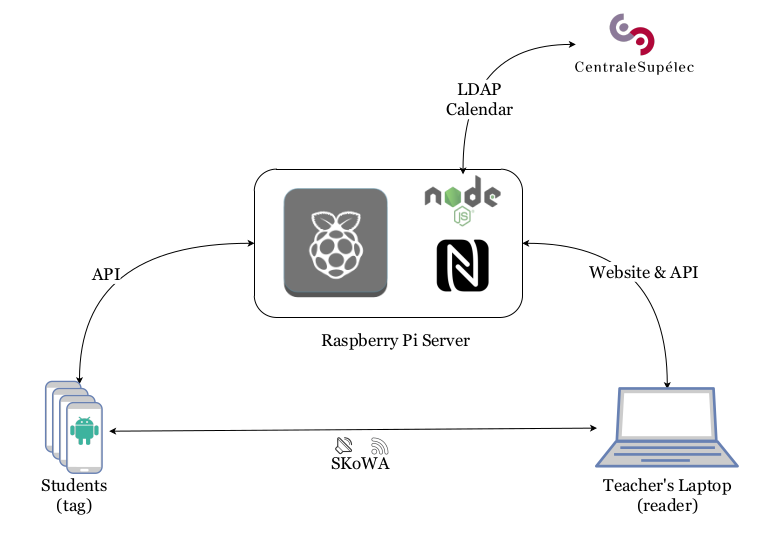
\includegraphics[height=0.8\textheight]{../assets/architecture.png}
\end{frame}


\section{Raspberry Pi}

\begin{frame}
    \frametitle{Sommaire}
    \tableofcontents[
      currentsection,
      sectionstyle=show/shaded,
      subsectionstyle=show/shaded/hide
    ]
\end{frame}

\begin{frame}{Présentation}
  Le raspberry Pi a plusieurs utilités dans notre projet, et sert de serveur pour certains composants.
  \begin{itemize}
    \item Lecteur NFC géré par une librairie python (NxpPy)
    \item Backend de l'application web (node JS)
    \item Base de donnée (SQLite3 pour le développement)
    \item Parsing du LDAP de CentraleSupélec puis écriture dans la DB
  \end{itemize}

  \begin{figure}
    \begin{subfigure}{.2\textwidth}
      \centering
      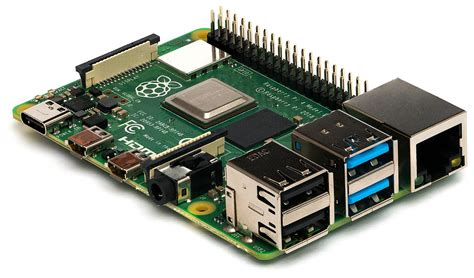
\includegraphics[width=.8\linewidth]{../assets/raspi.jpeg}
    \end{subfigure}
    \begin{subfigure}{.2\textwidth}
      \centering
      
\includegraphics[width=.8\linewidth]{../assets/nfc.png}
    \end{subfigure}
    \begin{subfigure}{.2\textwidth}
      \centering
      
\includegraphics[width=.8\linewidth]{../assets/nodejs.png}
    \end{subfigure}
  \end{figure}
\end{frame}

\subsection{NFC}

\begin{frame}{Présentation NFC}
  Nous avons utilisé le module \textit{explore-nfc} de la société NXP qui se branche sur les GPIO du raspberry PI
  \begin{figure}.
    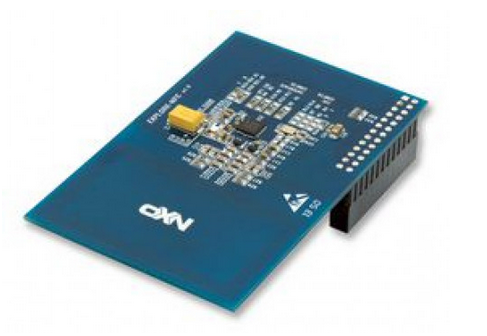
\includegraphics[width=.5\textwidth]{../assets/explorenfc.png}
  \end{figure}
\end{frame}

\begin{frame}{Fonctionnement du NFC}
  2 Scripts Python3 :
  \begin{itemize}
    \item Un script de polling qui interface avec le module NFC grâce à la librairie \textbf{NxpPY}, et qui communique avec le frontweb grâce à des websockets
    \item Un script \textit{Database Utils} qui interface avec la base de donnée \textbf{Sqlite3}
  \end{itemize}
  \begin{figure}
    \centering
    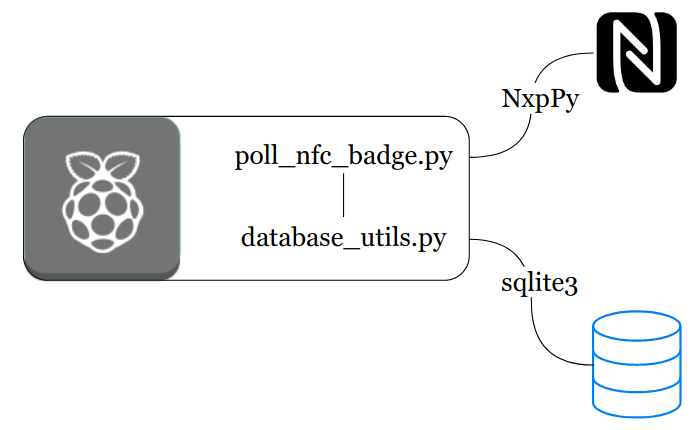
\includegraphics[width=.5\textwidth]{../assets/nfcarchitecture.png}
  \end{figure}
\end{frame}

\begin{frame}{poll\_nfc\_badge.py}
  Ce script utilise la librairie \textit{websockets} de Python3, qui est elle même basée sur \textit{asyncio} qui permet de faire de la programmation asynchrone
  C'est le front end qui envoie au serveur ce dont il a besoin :
  \begin{itemize}
    \item Type = 0 $\rightarrow$ Check Once (à l'ajout d'un utilisateur, permet de scanner le badge une fois)
    \item Type = 1 $\rightarrow$ Vérification à l'entrée dans l'amphi
    \item Type = 2 $\rightarrow$ Vérification à la sortie de l'amphi
  \end{itemize}

\end{frame}

\begin{frame}{Type 0 (Check Once)}
  \begin{figure}[]
    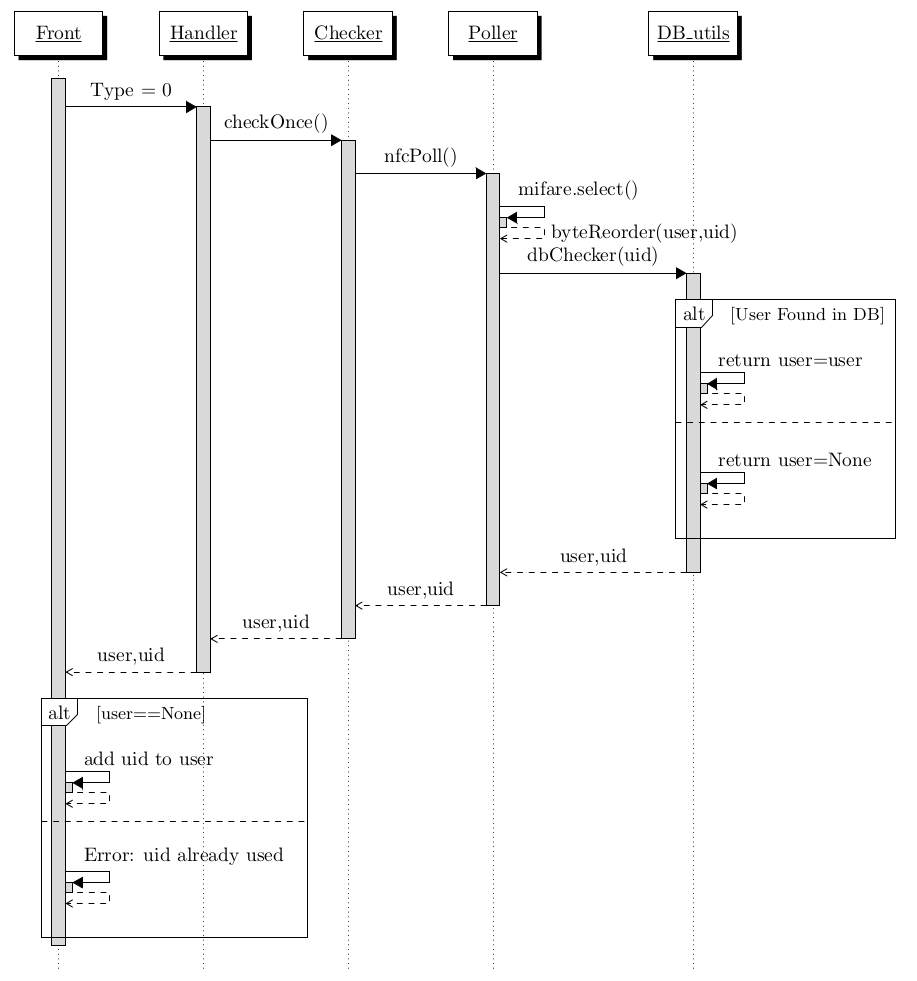
\includegraphics[height=.9\textheight]{../assets/nfcSeqOnce.png}
  \end{figure}
\end{frame}

\begin{frame}{Type 1 (Verification à l'entrée)}
  \begin{figure}[]
    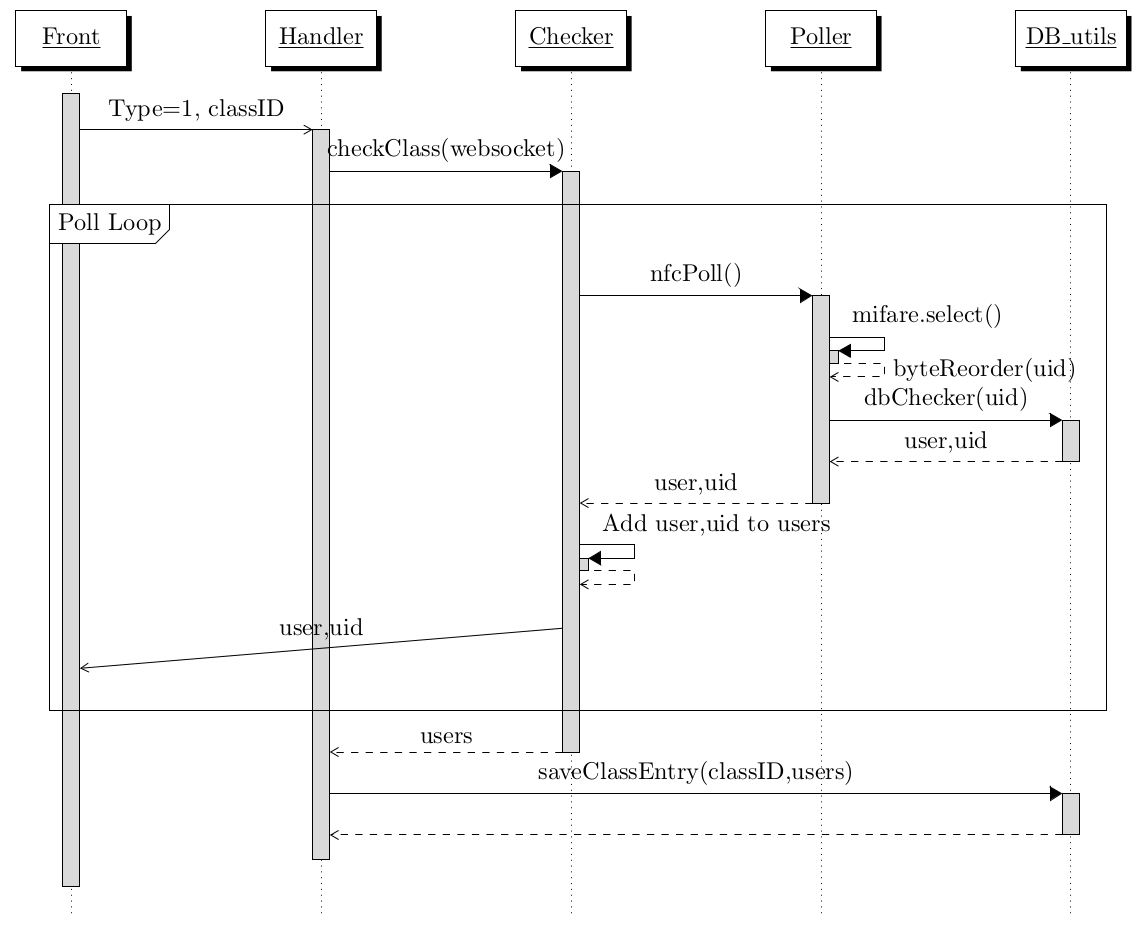
\includegraphics[height=.9\textheight]{../assets/nfcSeqEntry.png}
  \end{figure}
\end{frame}

\begin{frame}{Type 2 (Vérification à la sortie)}
  \begin{figure}[]
    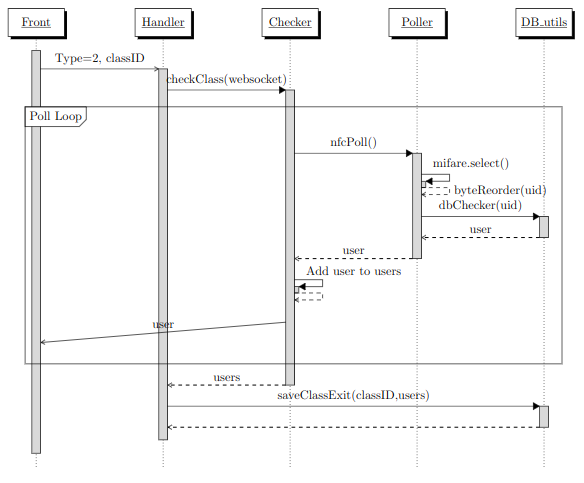
\includegraphics[height=.9\textheight]{../assets/nfcSeqExit.png}
  \end{figure}
\end{frame}

\subsection{Application Web}

\begin{frame}{Présentation de l'appli Web}
  Application web permettant de gérer les utilisateurs, et l'entrée et sortie d'amphi.
  \begin{itemize}
    \item Framework \textbf{Express JS} en \textbf{Node}
    \item Boostrap 4
    \item Connecteur Sqlite3 synchrone
    \item Connecteur aux scripts NFC par websockets
  \end{itemize}

  \begin{figure}
    \centering
    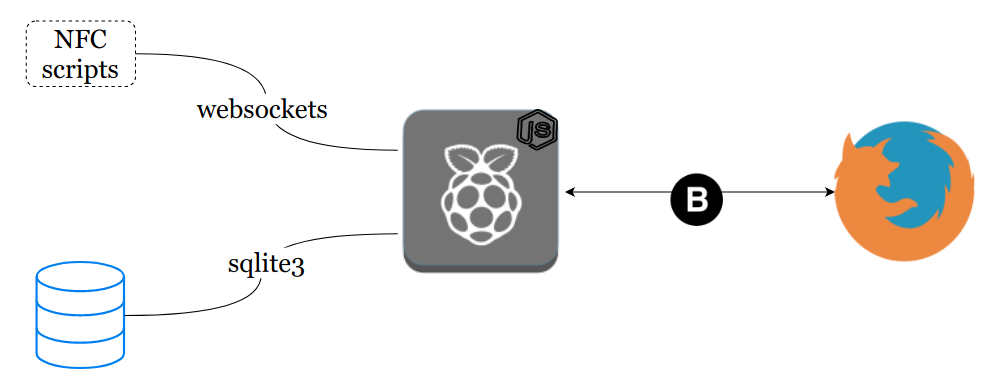
\includegraphics[width=.5\textwidth]{../assets/web_architecture.png}
  \end{figure}
\end{frame}

\begin{frame}{Structure de l'appli Web}
  3 pages principales :
  \begin{itemize}
    \item \textbf{Users :} Gestion des utilisateurs
    \item \textbf{Class :} Gestion de l'appel en Amphi
    \item \textbf{Presence :} Révision à posteriori de la présence
  \end{itemize}
\end{frame}

\begin{frame}{Démonstration}
  Voyons cela en live !
\end{frame}

\subsection{LDAP Parser}

\begin{frame}{Présentation du parser LDAP}
    Parser les fichier LDIF extraits du LDAP de l'école.
    \begin{itemize}
        \item Création des fichiers LDIF à partir du LDAP de l'école
        \item Utilisation de la librairie python-ldap
        \item Ecriture dans la BDD Sqlite3
    \end{itemize}
    \begin{figure}
        \centering
        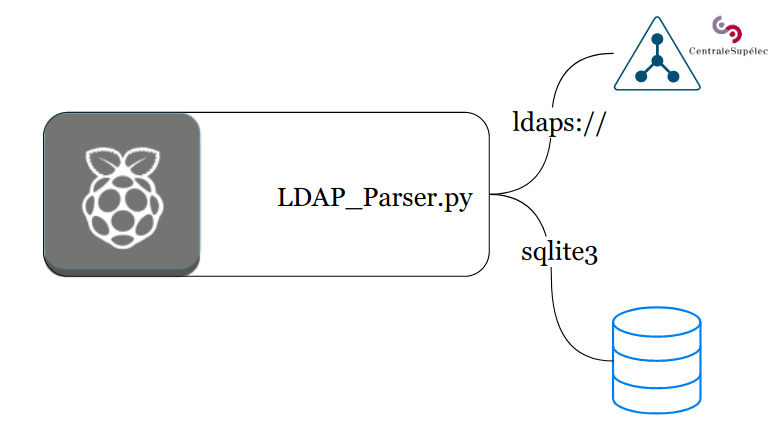
\includegraphics[width=.45\textwidth]{../assets/ldapparserarchitecture.png}
    \end{figure}
\end{frame}

\begin{frame}{Champs Récupérés}
   Voici les champs récupérés dès qu'ils existent dans le LDAP de l'école :
   \begin{itemize}
       \item cn (sous la forme \textit{Nom Prénom})
       \item lastname
       \item firstname
       \item username
       \item email
       \item badge\_id (l'ID NFC du badge étudiant ou de la carte pro)
       \item skowa\_id (un identifiant unique pour le SKoWA)
       \item affiliations (student, member, teacher, ...)
       \item primary\_affiliation (l'affiliation principale)
       \item nedap\_profile (student, employee)
       \item supann\_diplome (IS\_3A, ...)
       \item promotion (SIS, 2A, ...)
   \end{itemize}
\end{frame}

\begin{frame}{Récapitulatif de l'architecture}
    \begin{figure}
        \centering
        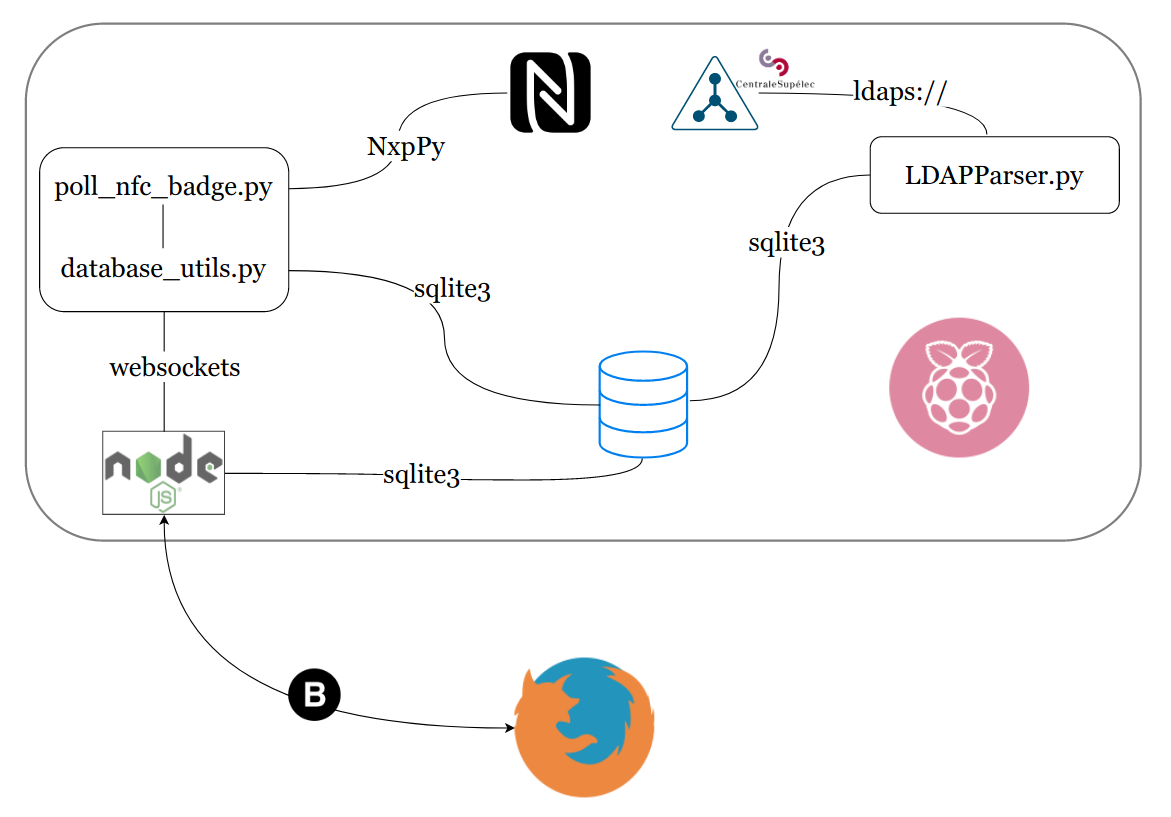
\includegraphics[width=.45\textwidth]{../assets/architectureraspberrypi.png}
    \end{figure}
\end{frame}

\section{SKoWA}

\subsection{Swiss-Knife}

\begin{frame}{Le protocole Swiss-Knife}
  Protocole délimiteur de distance proposé en 2008. \cite{SwissKnife}

  \bigskip

  \begin{itemize}
    \item Authentification
    \item Résistance aux mafia fraud et terrorist fraud
    \item Faible complexité algorithmique
    \item Faible taux de faux positifs
    \item Confidentialité
    \item Résistance aux erreurs
  \end{itemize}
\end{frame}

\begin{frame}{Le protocole Swiss-Knife}

  \centering
  \begin{tikzpicture}

    % Partie 1
    \draw (-3, 2) rectangle (3, 0.5);
    \node [above, blue] at (0, 1.25) {Phase de préparation};
    \node at (0, 1) {Initialisation, réponses};


    \draw (-3, 0) rectangle (3, -1.5);
    \node [above, blue] at (0, -0.75) {Phase rapide};
    \node at (0, -1) {$m$ questions / réponses};

    \draw (-3, -2) rectangle (3, -3.5);
    \node [above, blue] at (0, -2.75) {Phase de vérification};
    \node at (0, -3) {Vérification};

    \onslide<1->
  \end{tikzpicture}

\end{frame}

\begin{frame}{Librairie Swiss-Knife : Structure}
  \centering
  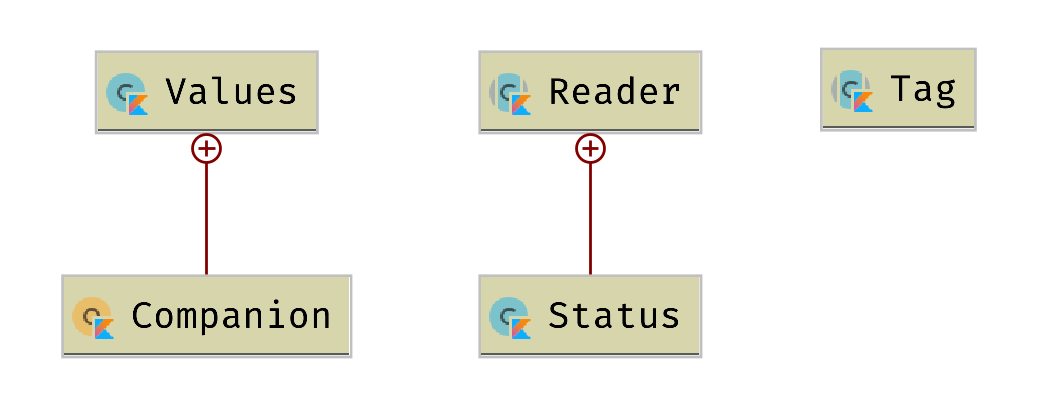
\includegraphics[width=.8\linewidth]{../assets/uml_jar.png}
\end{frame}

\begin{frame}{Phase de préparation}
  \begin{multicols}{2}
    \begin{minipage}[c]{\linewidth}
      \centering
      \bigskip
      \medskip
      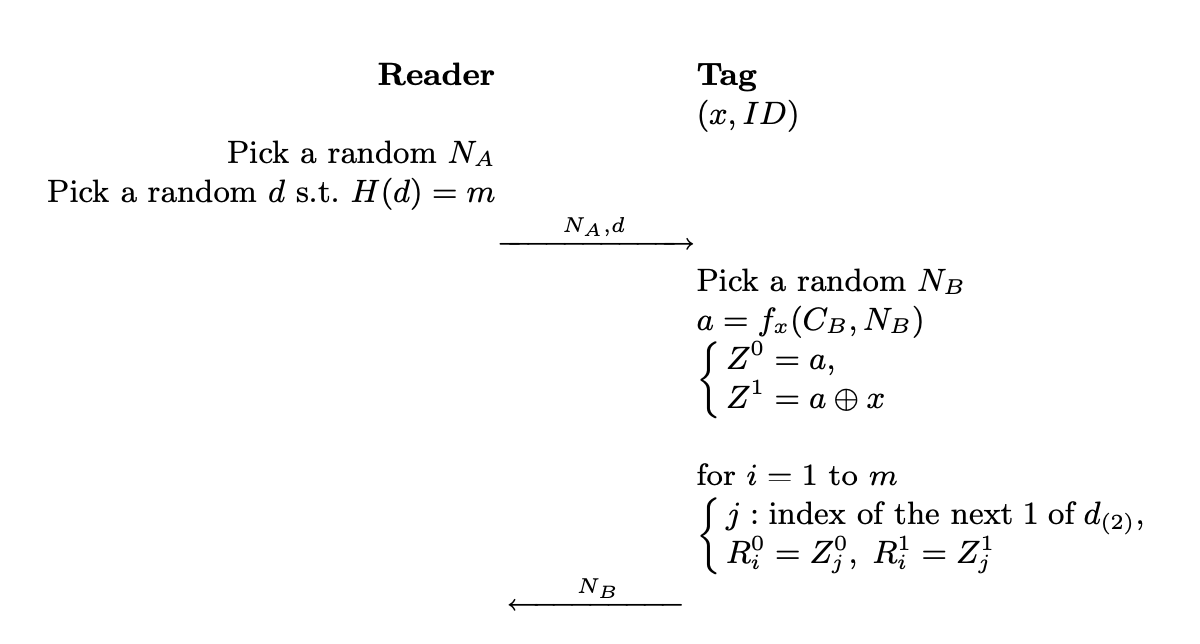
\includegraphics[width=\linewidth]{../assets/sk-phase1.png}
    \end{minipage}

    \begin{minipage}[t]{\linewidth}
      \begin{enumerate}
        \item Le lecteur choisit un nonce $N_A$, et $d$ un nombre avec $m$ bits 1.
        \item Le tag choisit un nonce $N_B$, et calcule $a = f_x(C_B, N_B)$ avec sa clé secrète $x$ et $N_B$. ($C_B$ est une constante)
        \item Le tag calcule $Z_0 = a$, $Z_1 = a \oplus x$. Il prépare ensuite les réponses possibles $R_0$ et $R_1$ selon le masque $d$.
        \item Le tag envoie $N_B$ au lecteur.
      \end{enumerate}
    \end{minipage}
  \end{multicols}
\end{frame}

\begin{frame}{Phase rapide}
  \begin{figure}[!htb]
    \centering

    \begin{minipage}{.45\textwidth}
      \centering
      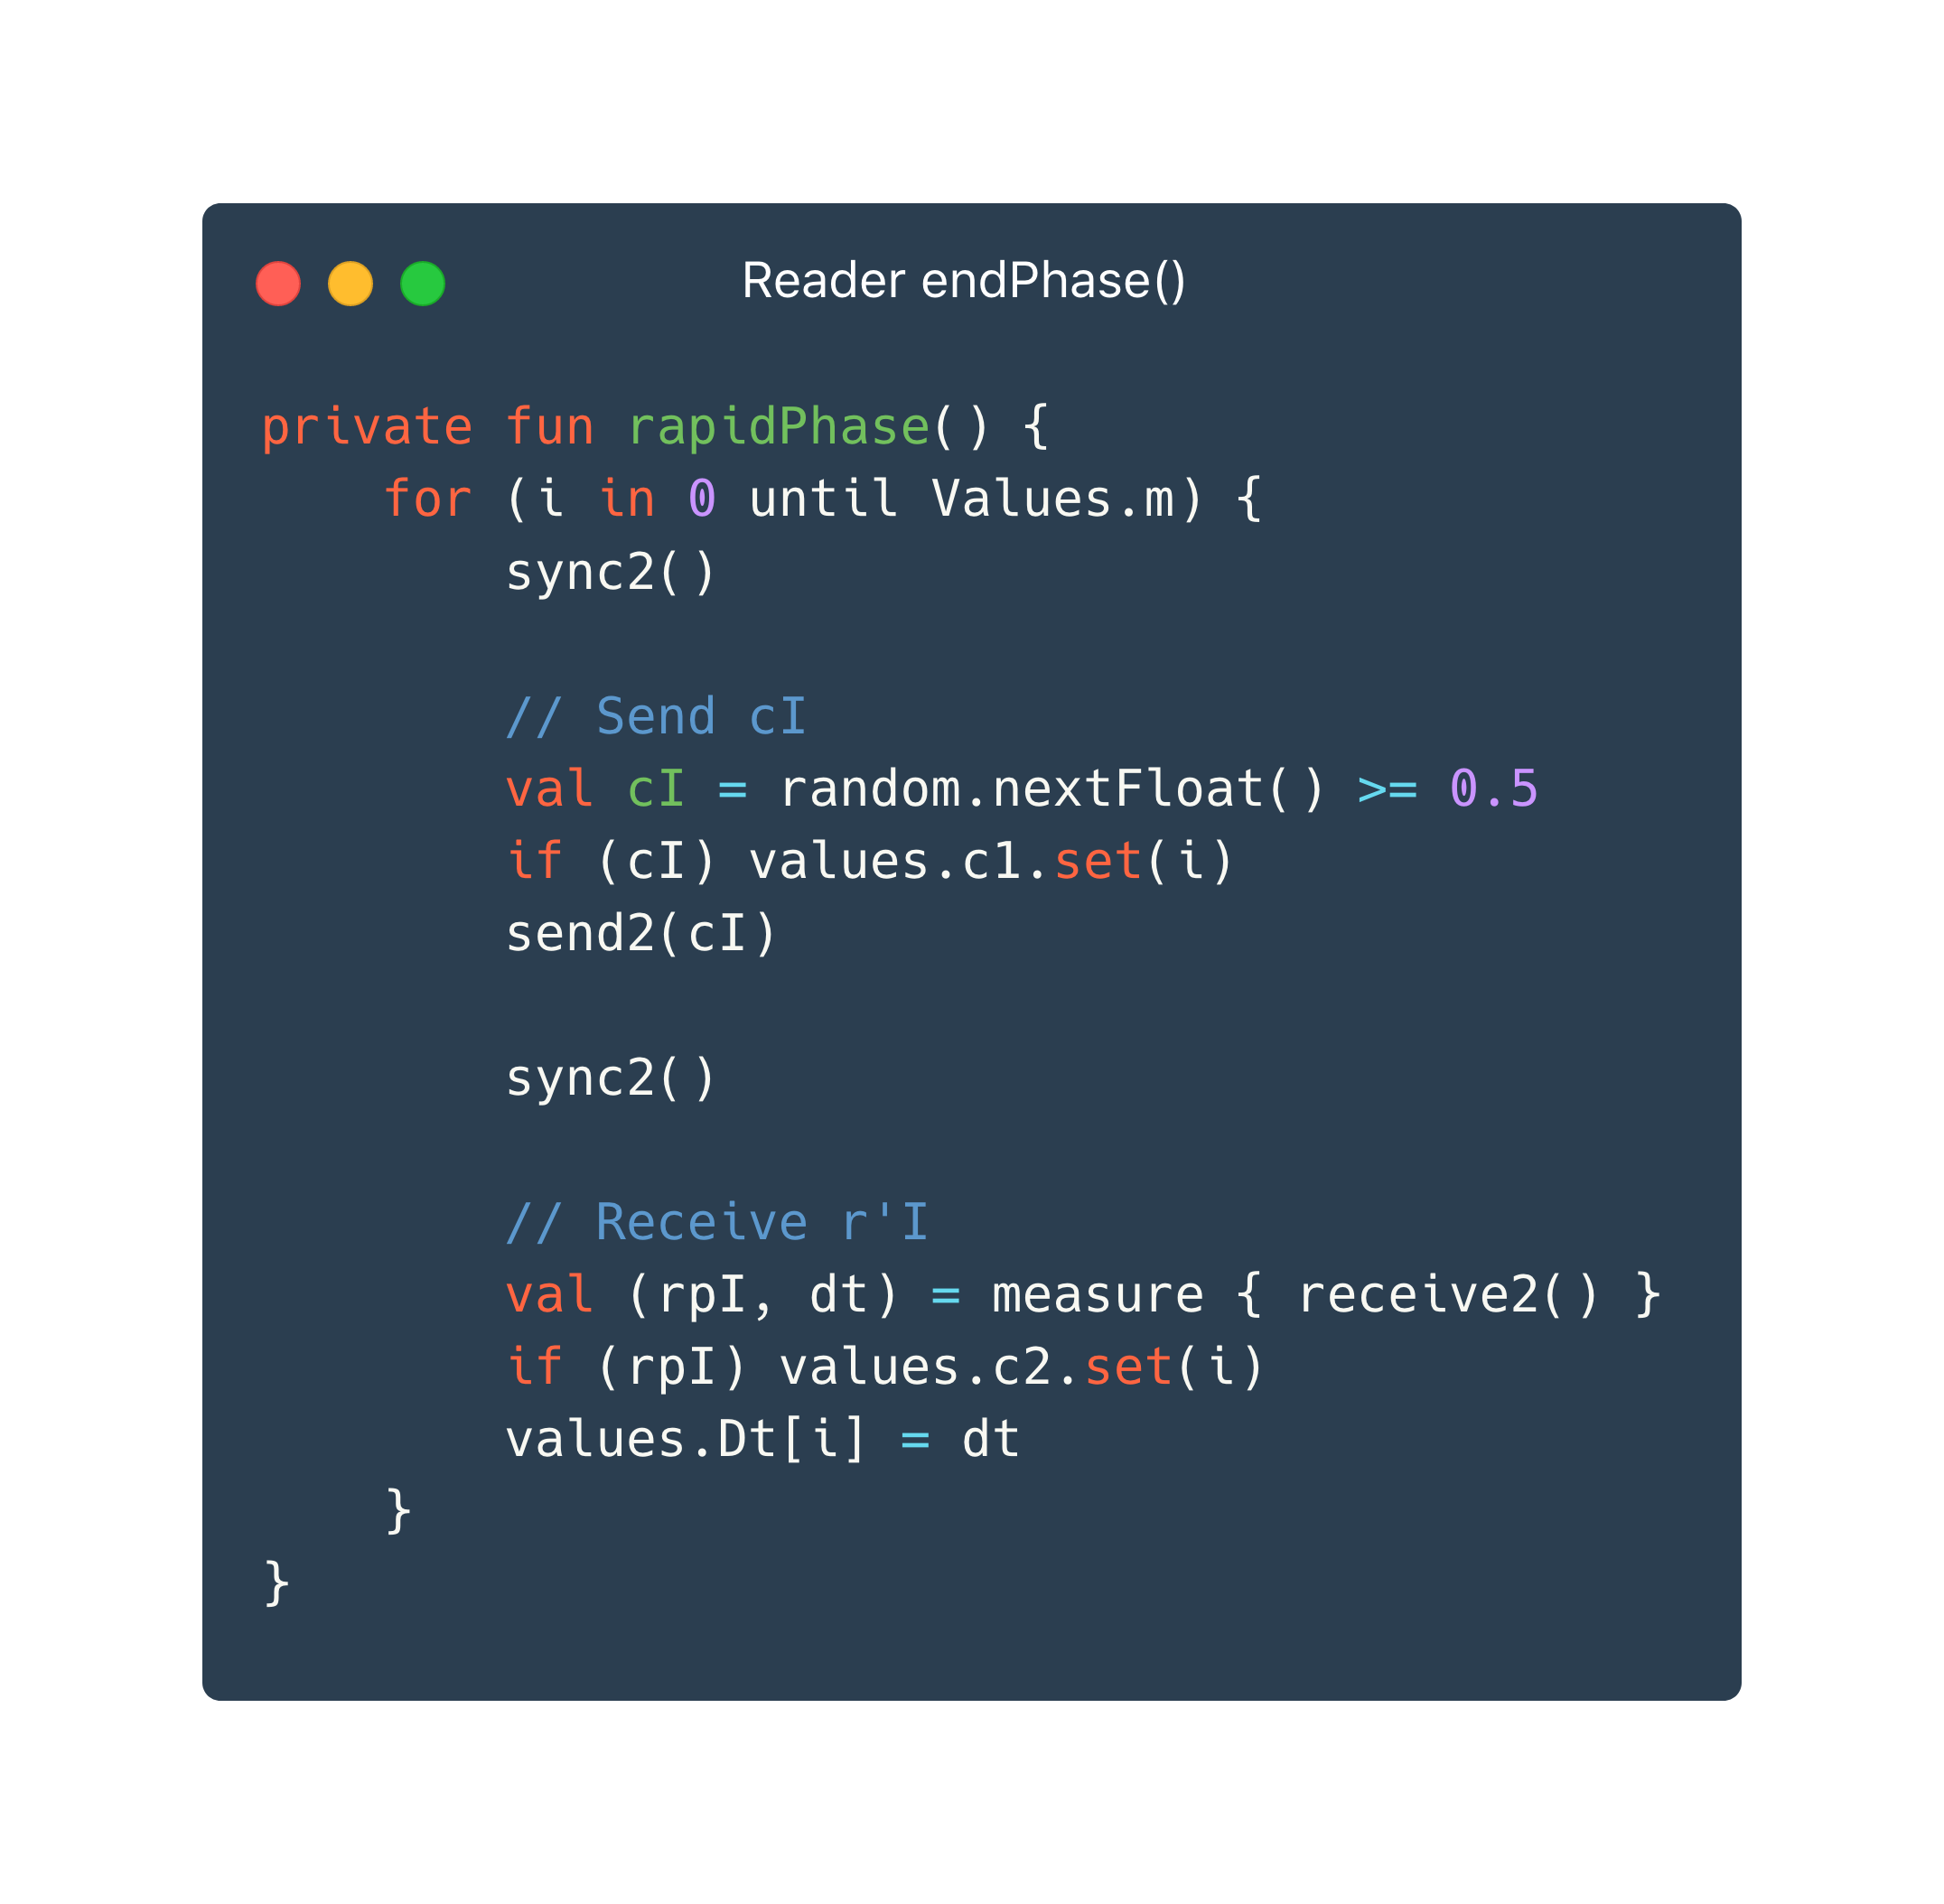
\includegraphics[width=\linewidth]{../assets/reader2}
    \end{minipage}%
    \begin{minipage}{.55\textwidth}
      \centering
      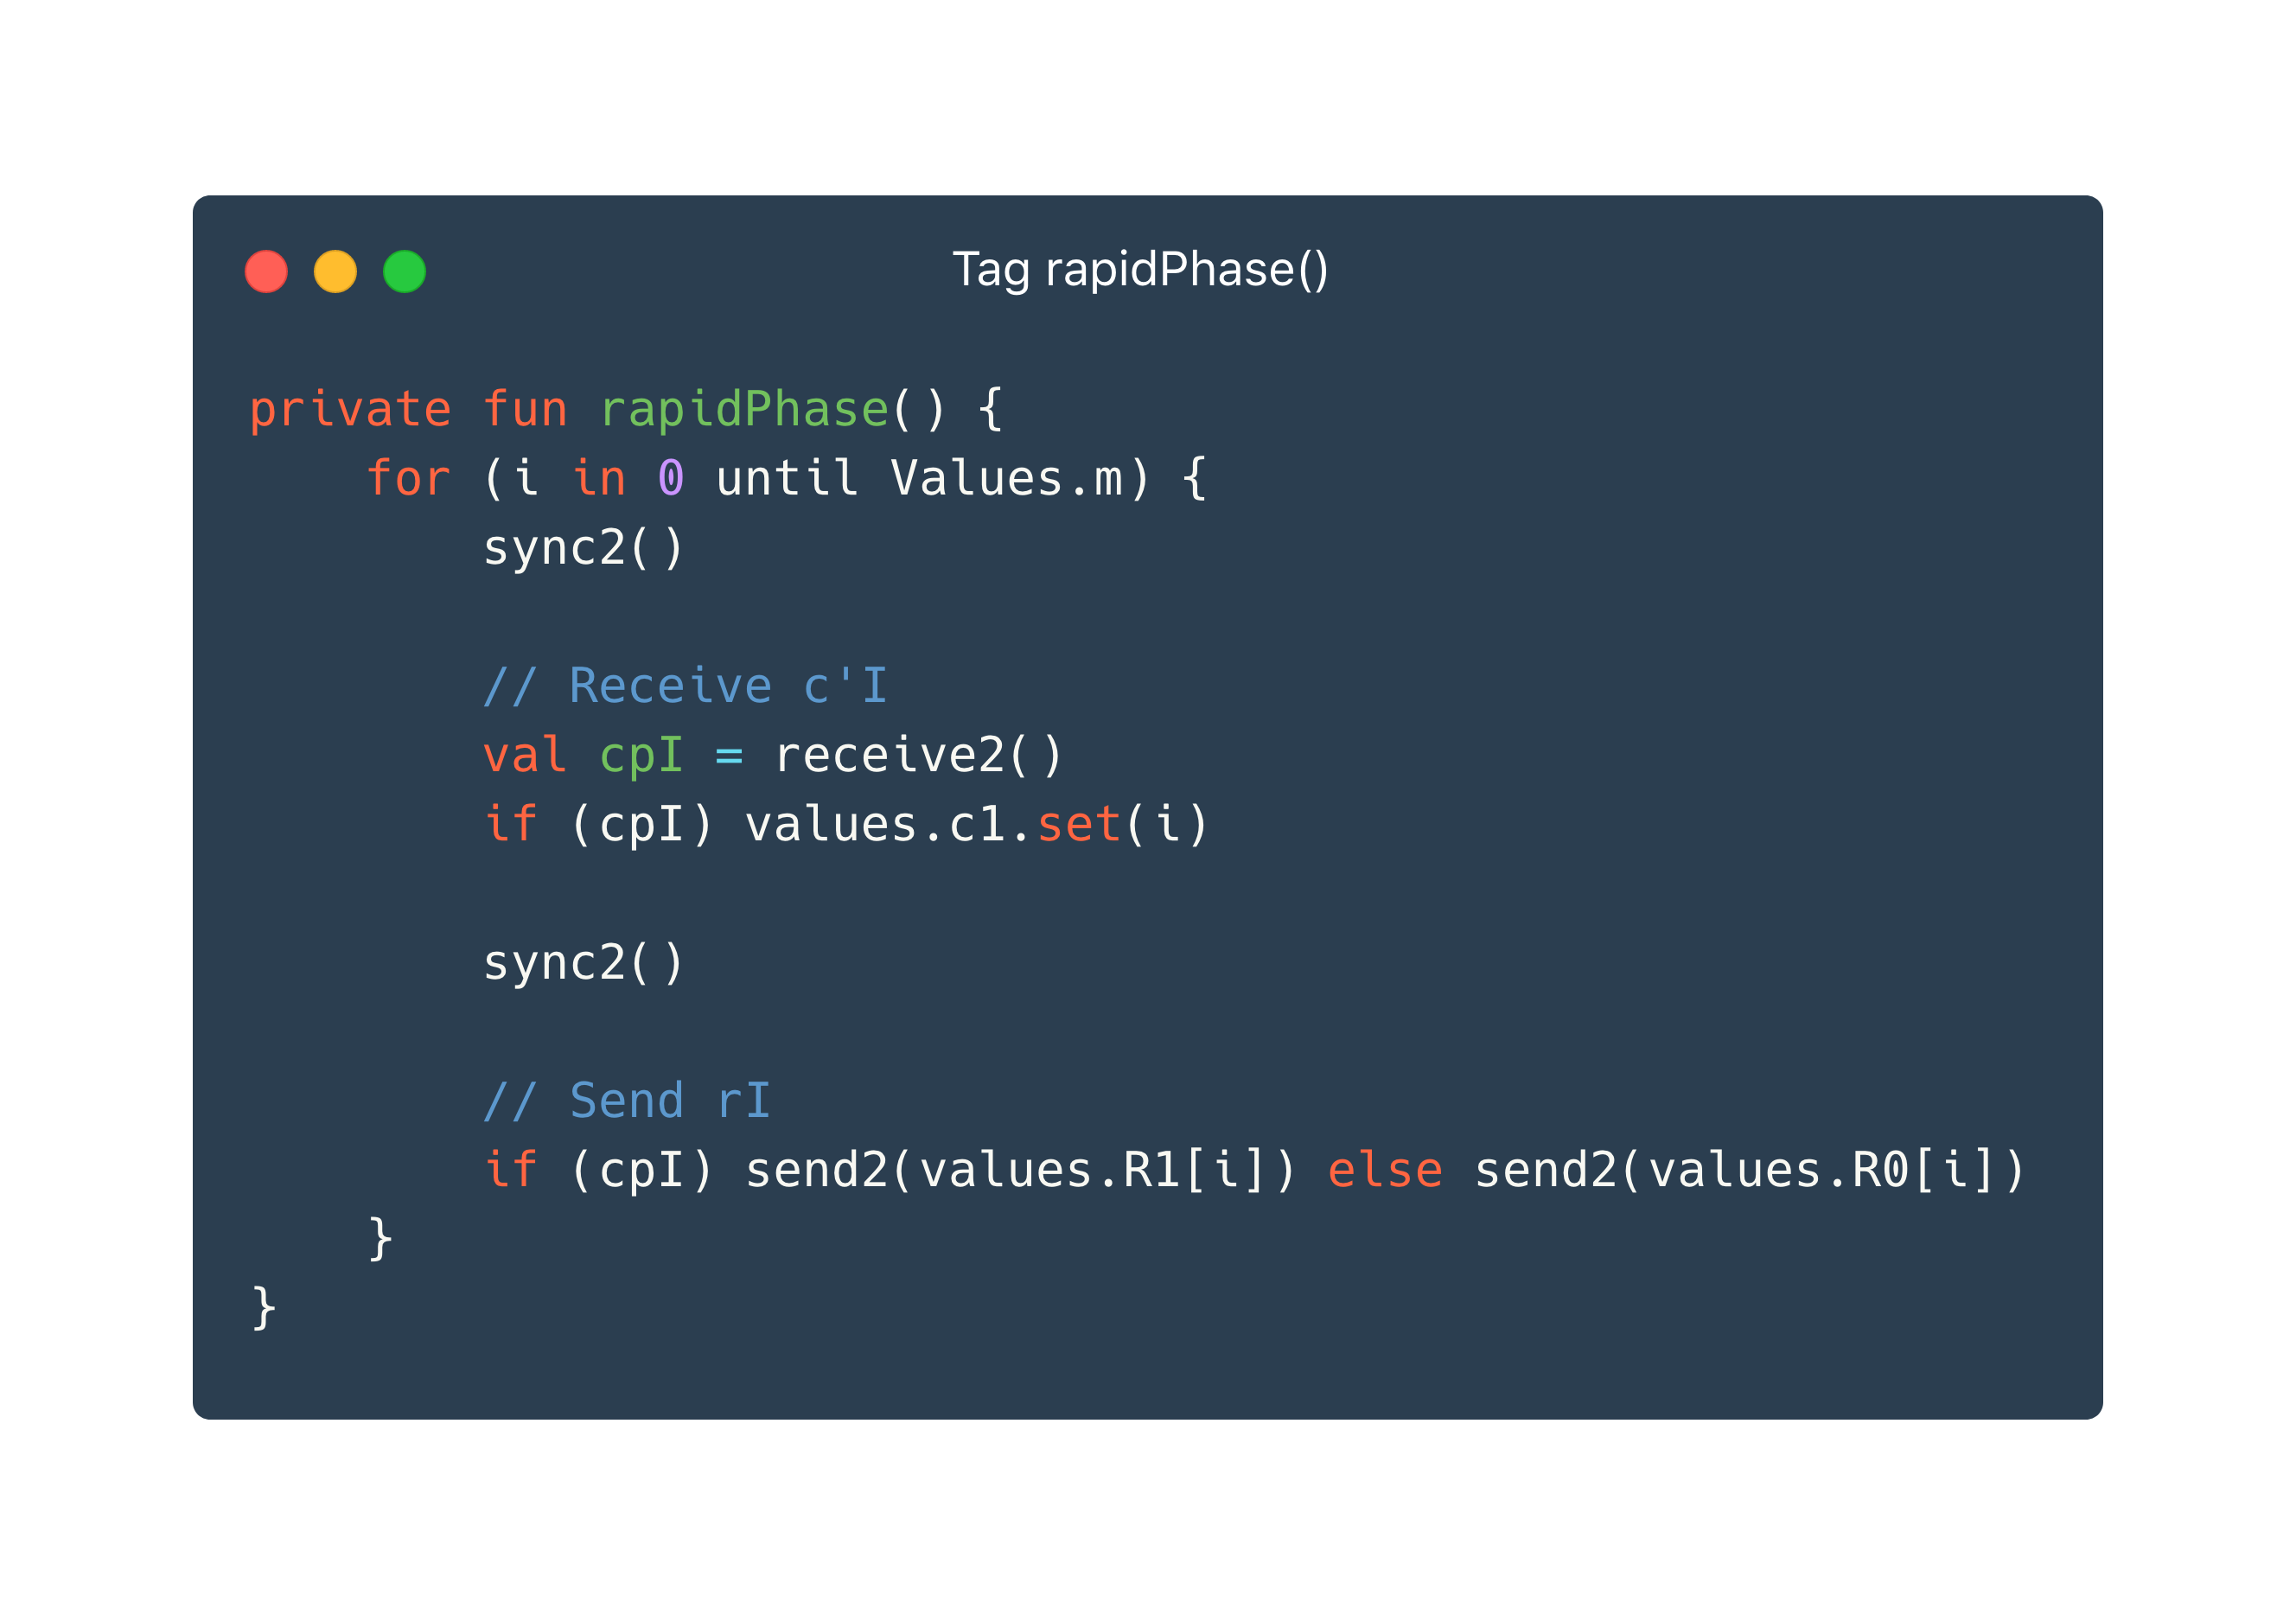
\includegraphics[width=\linewidth]{../assets/tag2}
    \end{minipage}

  \end{figure}
\end{frame}

\begin{frame}{Phase de vérification}
  \begin{multicols}{2}
    \begin{minipage}[c]{\linewidth}
      \centering
      \bigskip
      \bigskip
      \bigskip
      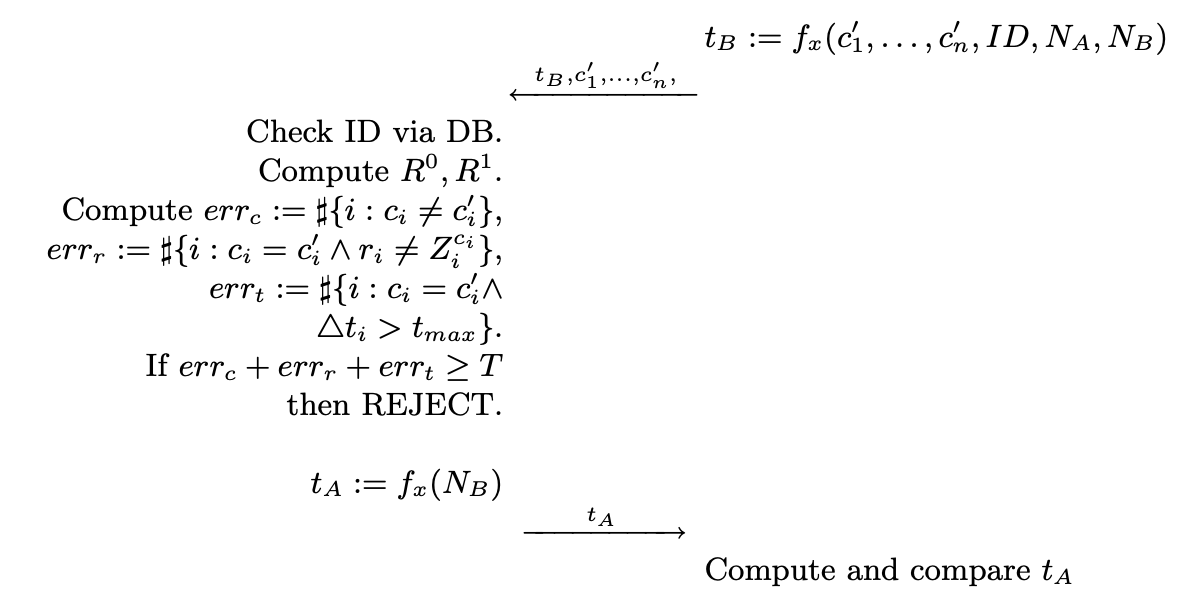
\includegraphics[width=\linewidth]{../assets/sk-phase3}
    \end{minipage}

    \begin{minipage}[t]{\linewidth}
      \begin{enumerate}
        \item Le tag envoie $t_B = f_x(c'_1, \hdots, c'_n, ID, N_A, N_B)$, et les $c'_i$.
        \item Le lecteur cherche dans sa base de tags jusqu'à trouver $(ID, x)$ générant $t_B$.
        \item Le lecteur calcule $R^0$ et $R^1$.
        \item Le lecteur compte les erreurs, si il y en a plus de $T$, échec.
        \item (optionnel) Le lecteur envoie $t_A := f_x(N_B)$ puis le tag le vérifie.
      \end{enumerate}
    \end{minipage}
  \end{multicols}
\end{frame}

\begin{frame}{Librairie Swiss-Knife : Test unitaire}
  \centering
  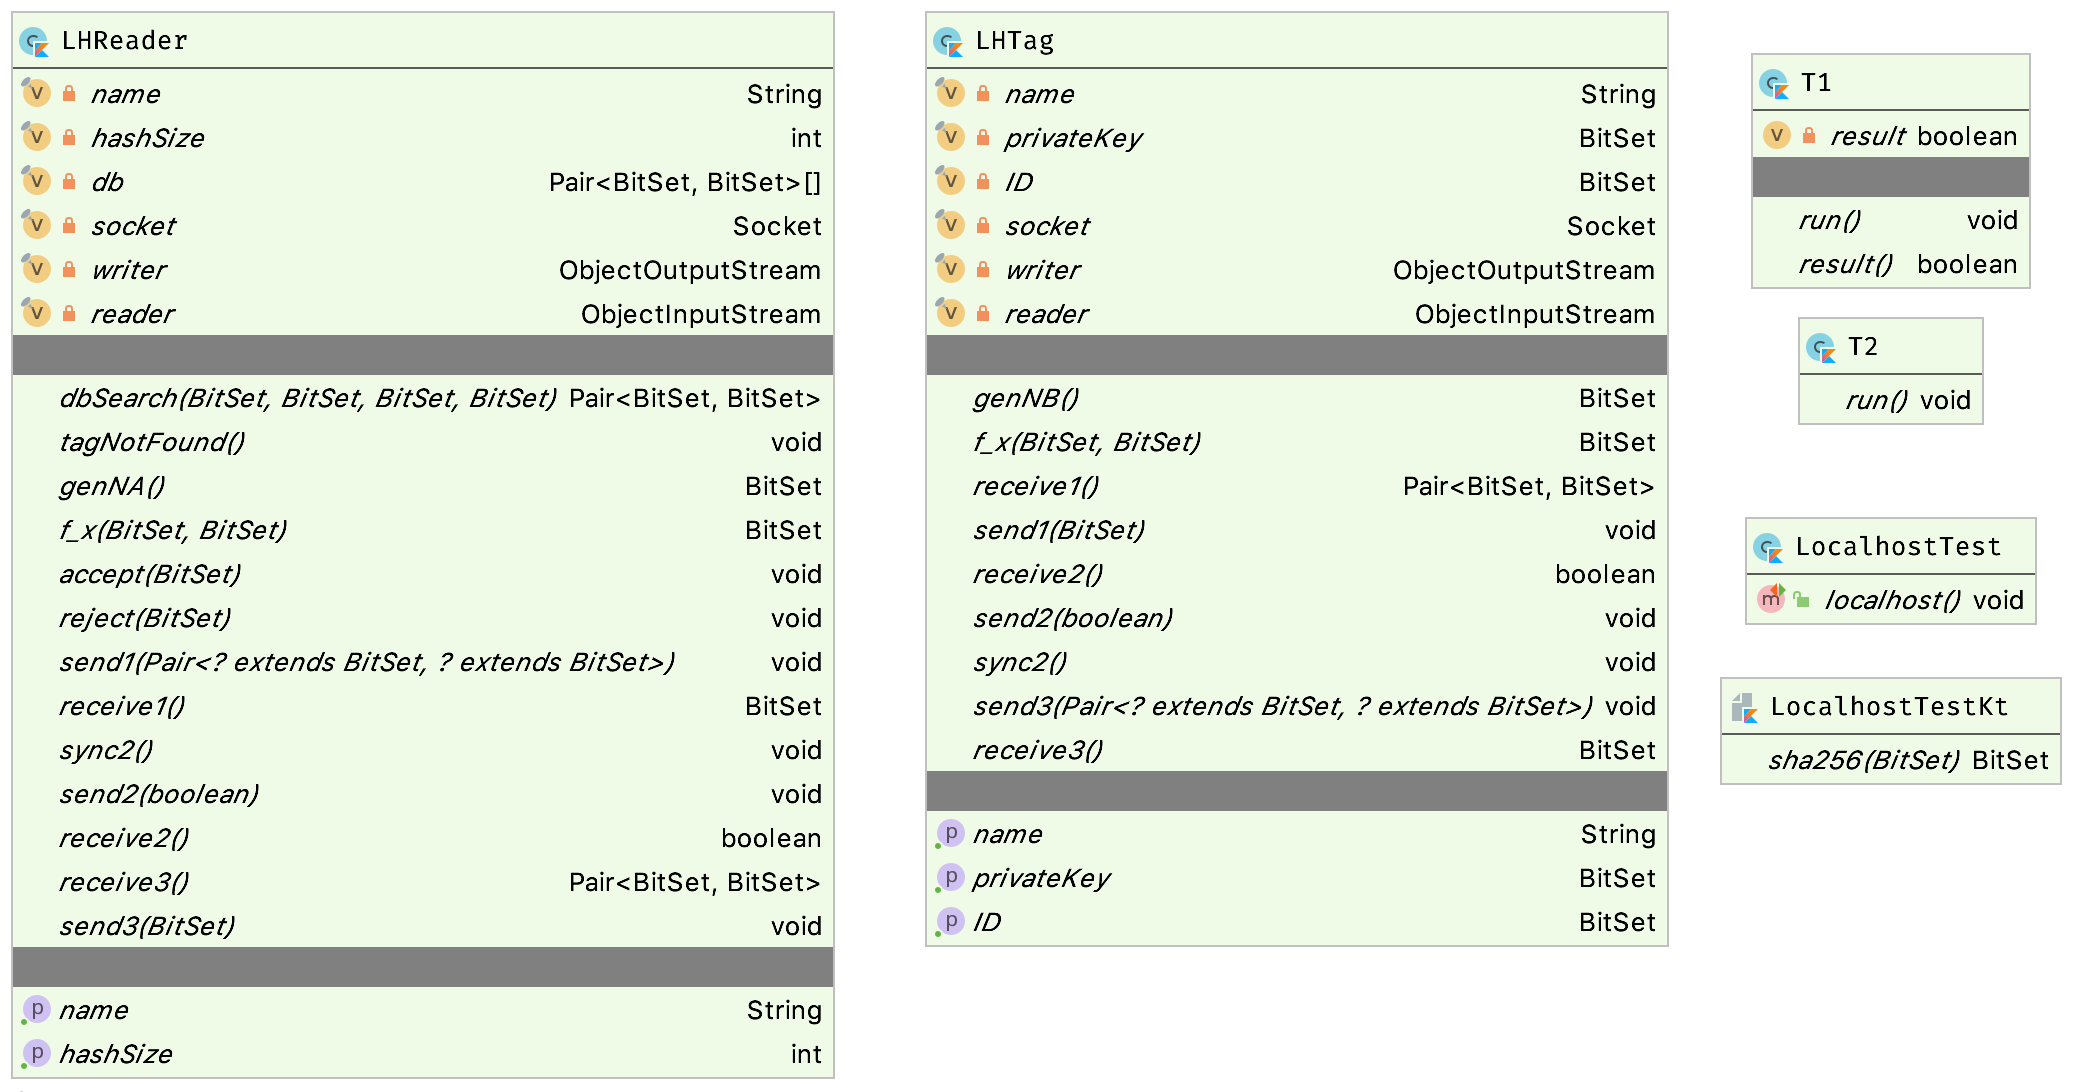
\includegraphics[height=.9\textheight]{../assets/uml_test_detail}
\end{frame}

\begin{frame}{Librairie Swiss-Knife : Notre utilisation}
  SKoWA : Swiss-Knife Over Wi-Fi and Audio
  \bigskip

  \begin{itemize}
    \item On utilise un socket pour les phases 1 et 3
    \item On utilise du son pour la phase 2
  \end{itemize}
\end{frame}

\subsection{SKoWA Tag \& Reader}

\begin{frame}{Application Android}

  \begin{itemize}
    \item Voir ses cours de la journée
    \item Adhérer à la vérification de présence
    \item Effectuer le SKoWA (tag)
  \end{itemize}

\end{frame}

\begin{frame}{Maquette de l'application}
  \begin{adjustwidth}{-1.8em}{2em}
    \centering
    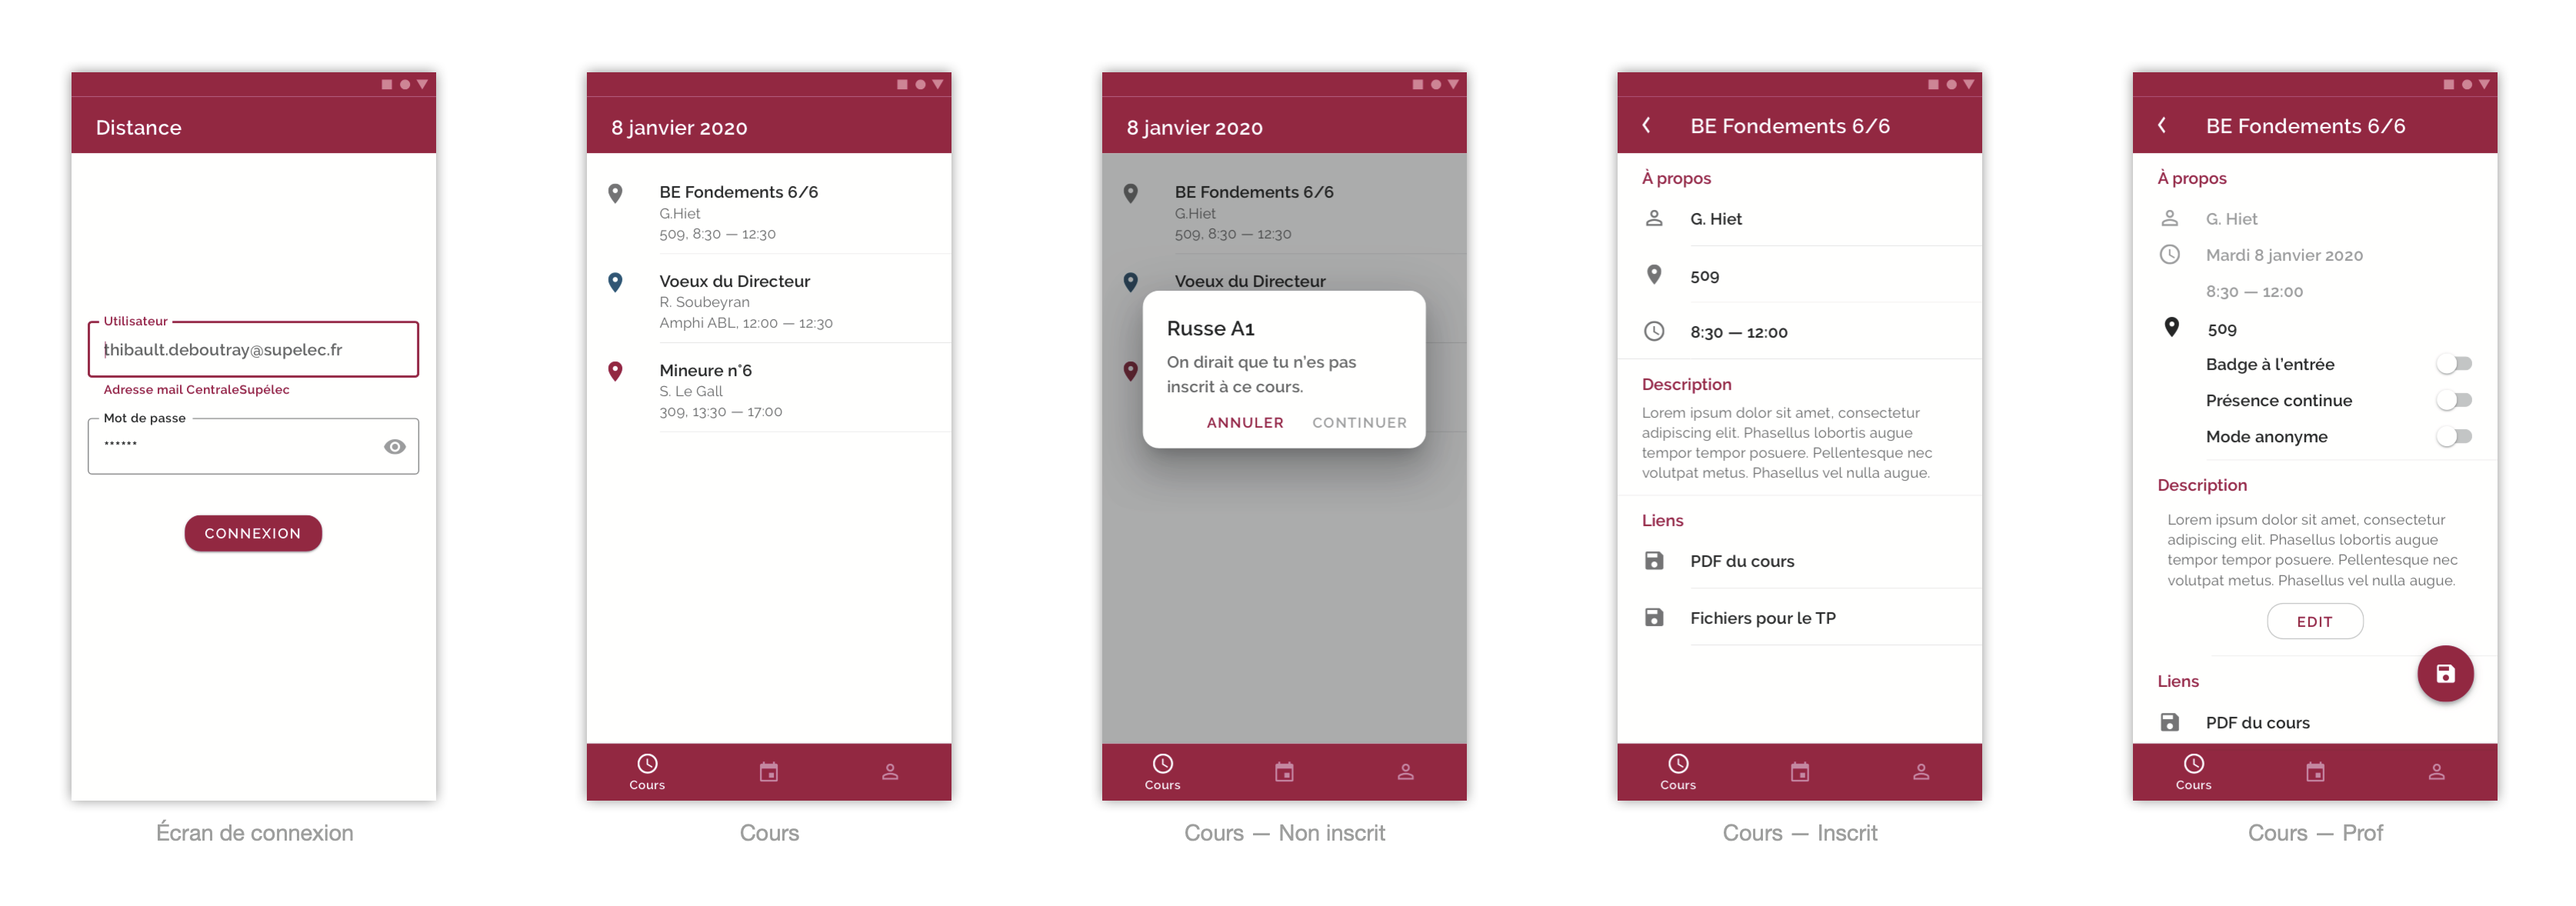
\includegraphics[width=1.1\textwidth]{../assets/maquette.png}
  \end{adjustwidth}
\end{frame}

\begin{frame}{App actuelle}

  \begin{minipage}{.4\textwidth}
    \begin{itemize}
      \item Liste de cours (custom RecyclerView / Adapter)
      \item Test Audio
      \item SKoWA tag
    \end{itemize}
  \end{minipage}%
  \begin{minipage}{.3\textwidth}
    \centering
    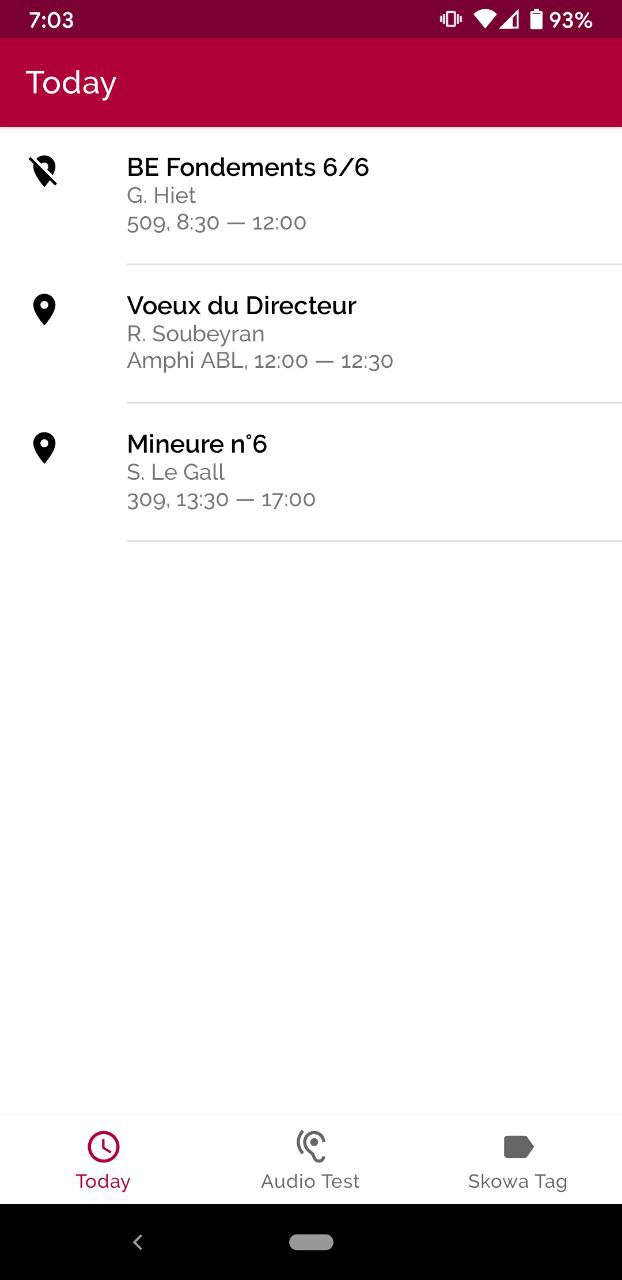
\includegraphics[height=.8\textheight]{../assets/android1}
  \end{minipage}%
  \begin{minipage}{.3\textwidth}
    \centering
    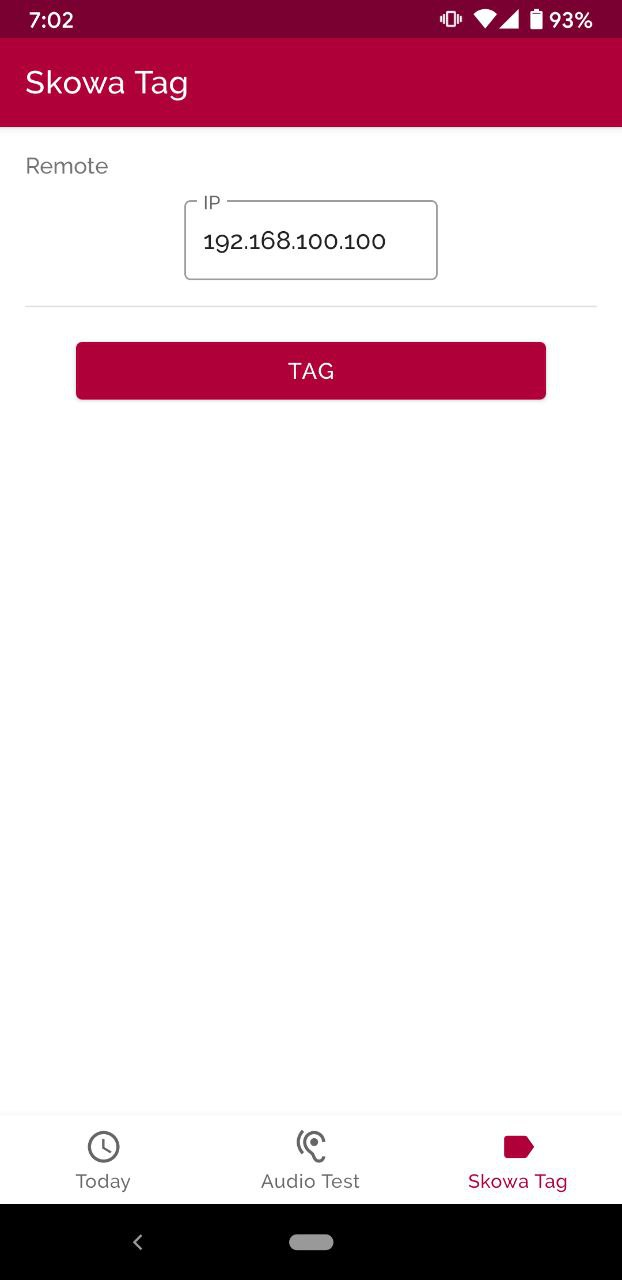
\includegraphics[height=.8\textheight]{../assets/android2}
  \end{minipage}

\end{frame}


\begin{frame}{Traitement du signal}
  \centering
  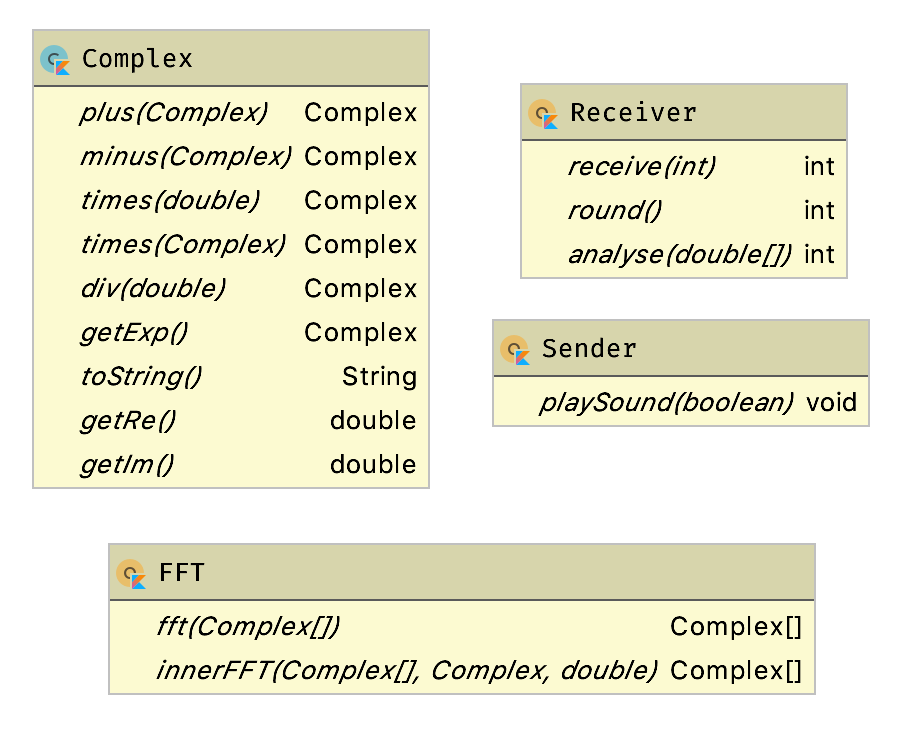
\includegraphics[height=.9\textheight]{../assets/uml_signal}
\end{frame}

\begin{frame}{Traitement du signal : rounds}
  \centering
  \begin{tikzpicture}

    \draw (-3, 1) rectangle (-1, 0);
    \node at (-2, 0.5) {-1};

    \draw (-1, 1) rectangle (1, 0);
    \node at (0, 0.5) {-1};

    \draw (1, 1) rectangle (3, 0);
    \node [blue] at (2, 0.5) {1};

    \draw (3, 1) rectangle (5, 0);
    \node at (4, 0.5) {};

    \onslide<1->
  \end{tikzpicture}

  \medskip

  \begin{tikzpicture}

    \draw (-3, 1) rectangle (-1, 0);
    \node at (-2, 0.5) {-1};

    \draw (-1, 1) rectangle (1, 0);
    \node [blue] at (0, 0.5) {0};

    \draw (1, 1) rectangle (3, 0);
    \node at (2, 0.5) {};

    \draw (3, 1) rectangle (5, 0);
    \node at (4, 0.5) {};

    \onslide<1->
  \end{tikzpicture}

  \medskip

  \begin{tikzpicture}

    \draw (-3, 1) rectangle (-1, 0);
    \node at (-2, 0.5) {-1};

    \draw (-1, 1) rectangle (1, 0);
    \node at (0, 0.5) {-1};

    \draw (1, 1) rectangle (3, 0);
    \node at (2, 0.5) {-1};

    \draw (3, 1) rectangle (5, 0);
    \node [red] at (4, 0.5) {-1};

    \onslide<1->
  \end{tikzpicture}
\end{frame}

\begin{frame}{SKoWA}
  \begin{minipage}{.4\textwidth}
    \centering
    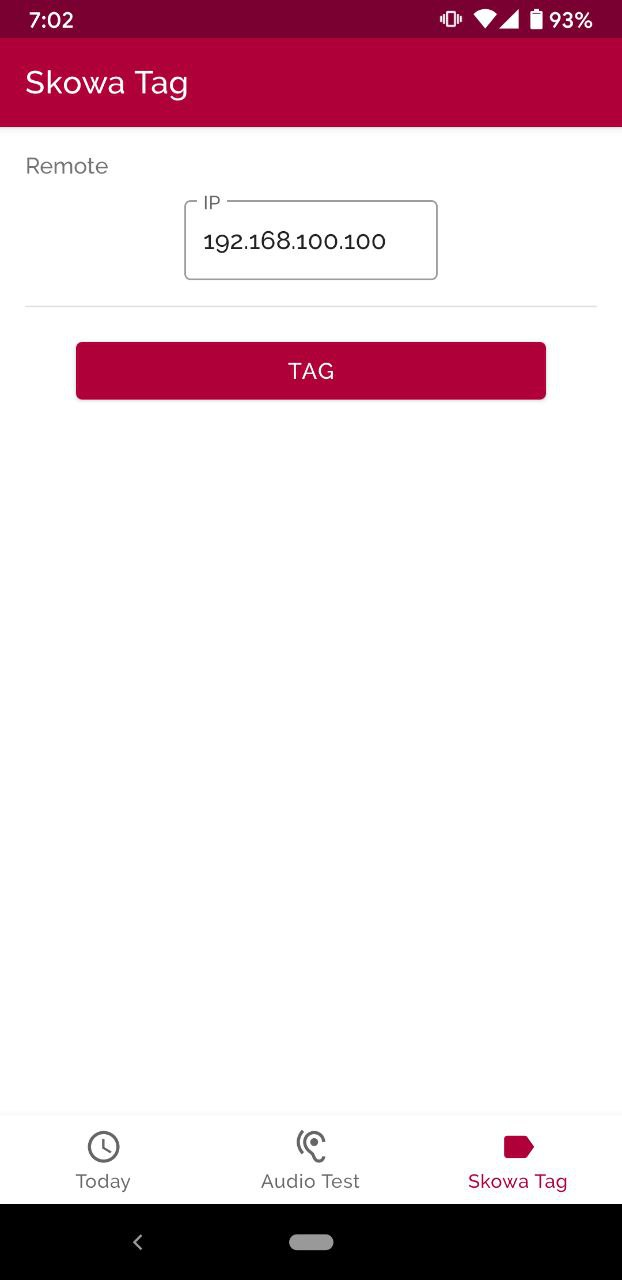
\includegraphics[height=.8\textheight]{../assets/android2}
  \end{minipage}%
  \begin{minipage}{.6\textwidth}
    \centering
    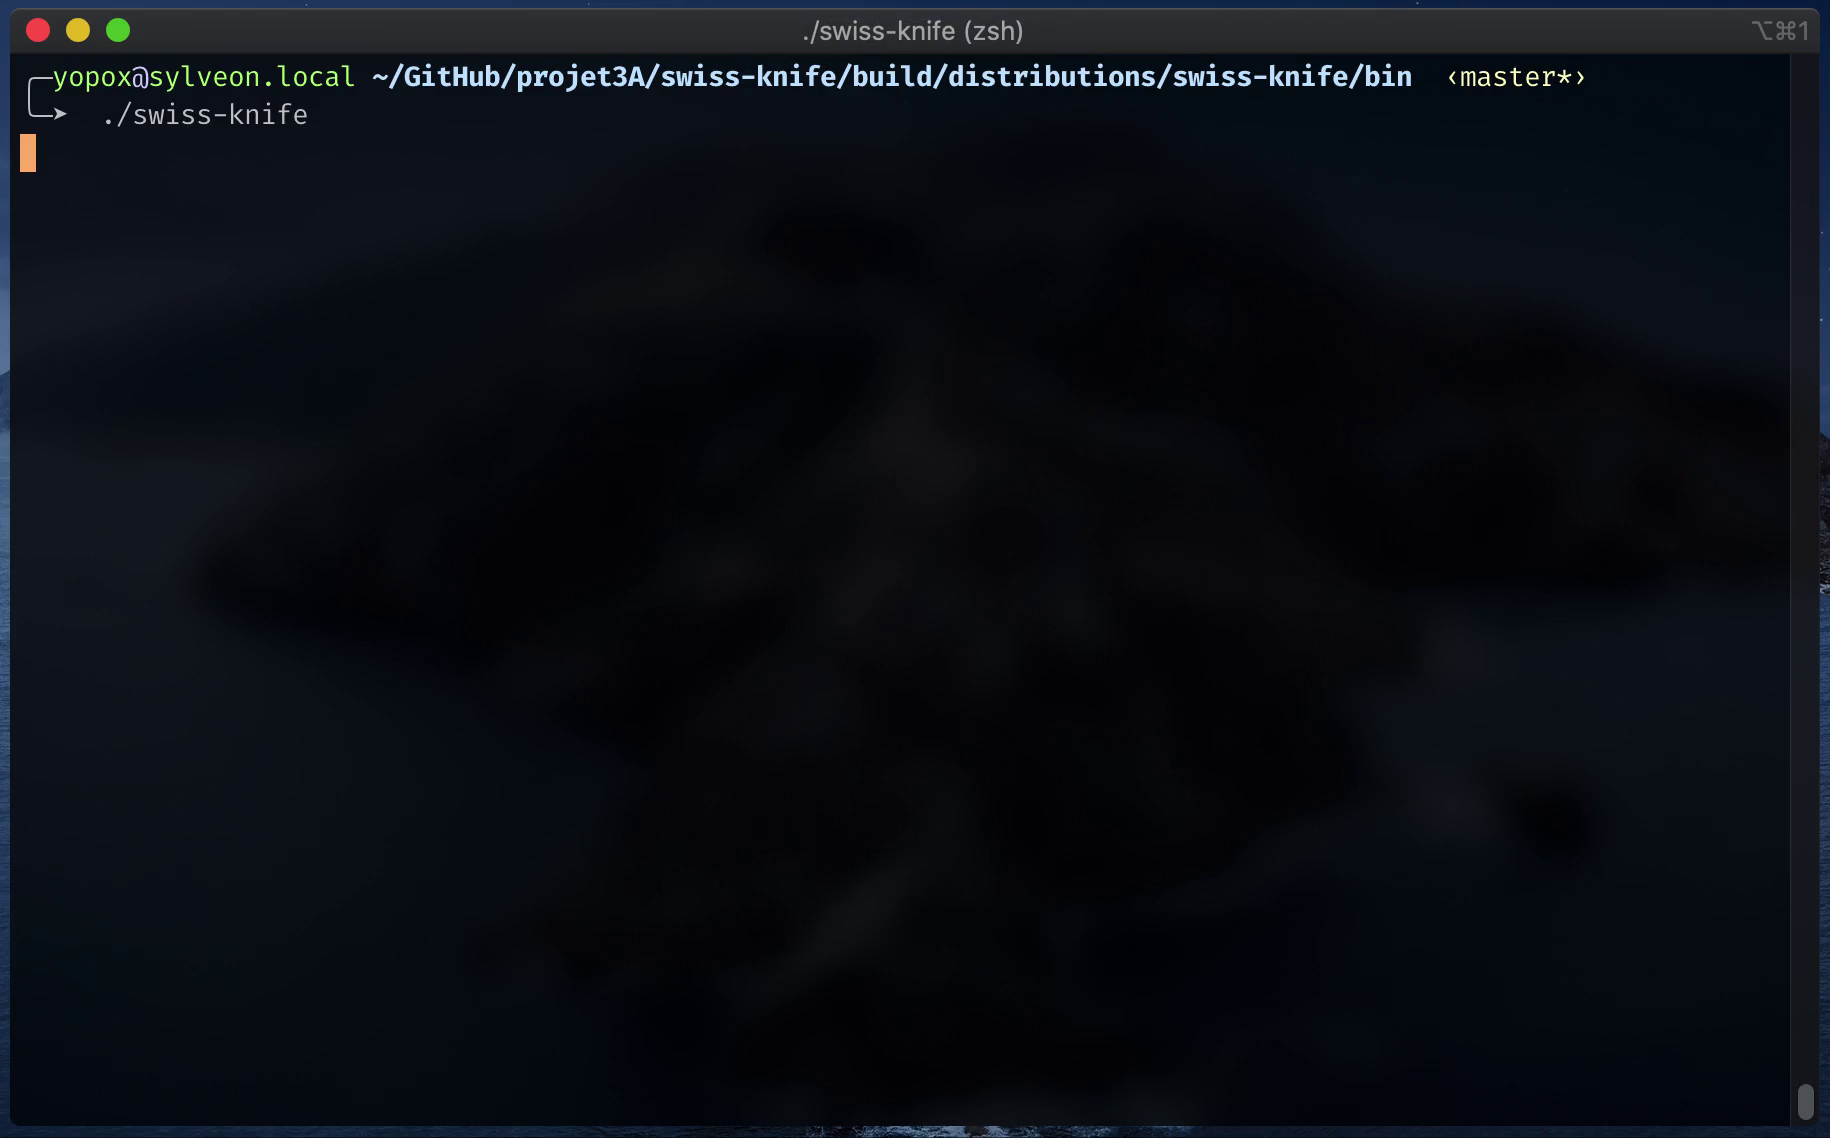
\includegraphics[width=\textwidth]{../assets/skowa-reader}
  \end{minipage}
\end{frame}

\section{Perspectives}

\begin{frame}
  \begin{figure}
    \centering
    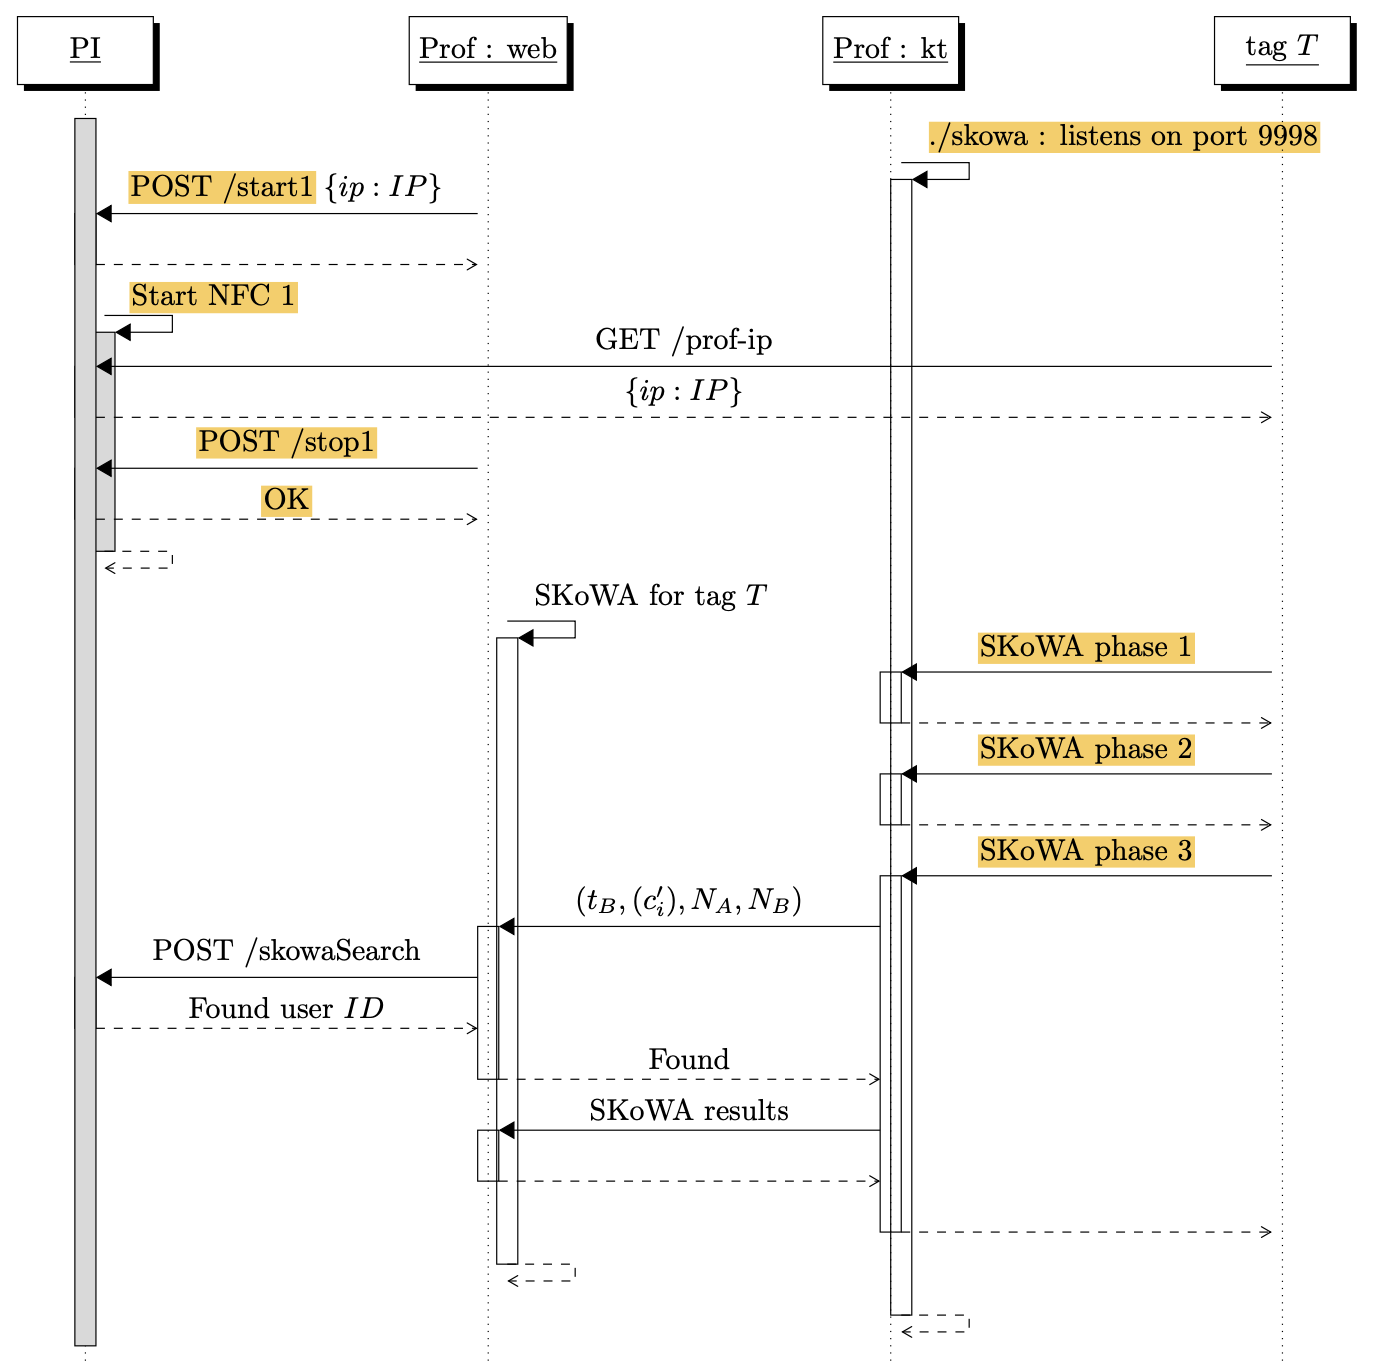
\includegraphics[height=.9\textheight]{../assets/seq.png}
    \captionsetup{labelformat=empty}
    \caption{Mise en commun : diagramme de séquence}
  \end{figure}
\end{frame}

\begin{frame}{Pour continuer...}

  \begin{itemize}
    \item Améliorer le traitement du signal
    \item Mettre en commun la partie NFC et le SKoWA
    \item Vérifier les nouvelles normes Wi-Fi
    \item Finaliser l'application Android
    \item Améliorer le filtrage de l'interface web
    \item Améliorer l'ergonomie générale de l'interface web (user friendliness)
    \item Intégrer le calendrier de l'école pour chaque User
  \end{itemize}  

\end{frame}

\section{Conclusion}

\begin{frame}{Conclusion}
  Projet très vaste, beaucoup de facettes pas forcément simples à interfacer.
  
  \bigskip
  
  On a touché à plein de choses ! La preuve :
  \begin{figure}
    \centering
    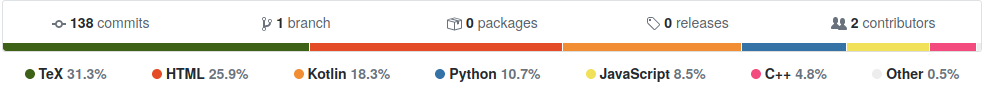
\includegraphics[width=\textwidth]{../assets/languages.png}
  \end{figure}
\end{frame}

\begin{frame}{Références}
  \printbibliography
\end{frame}

%%%%%%%%%%%%%%%%%%%%%%%%%%%%%%%%%%%%%%%%%%%%%%%%%%%%%%%%%%%
%%%%%%%%%%%%%%%%%%   Appendix   %%%%%%%%%%%%%%%%%%%%%%%%%%%
%%%%%%%%%%%%%%%%%%%%%%%%%%%%%%%%%%%%%%%%%%%%%%%%%%%%%%%%%%%

\section*{Annexes}

\appendix

% Renew toc command
\AtBeginSection[]
{
  \begin{frame}
    \frametitle{Sommaire des Annexes}
    \tableofcontents[
        currentsection,
        sectionstyle=show/shaded,
        subsectionstyle=show/shaded/hide
    ]
    \end{frame}
}

% Title Page
\begin{frame}
  \centering \Huge 
  Annexes
\end{frame}

\section{Appli web}

\begin{frame}
  \begin{figure}
    \centering
    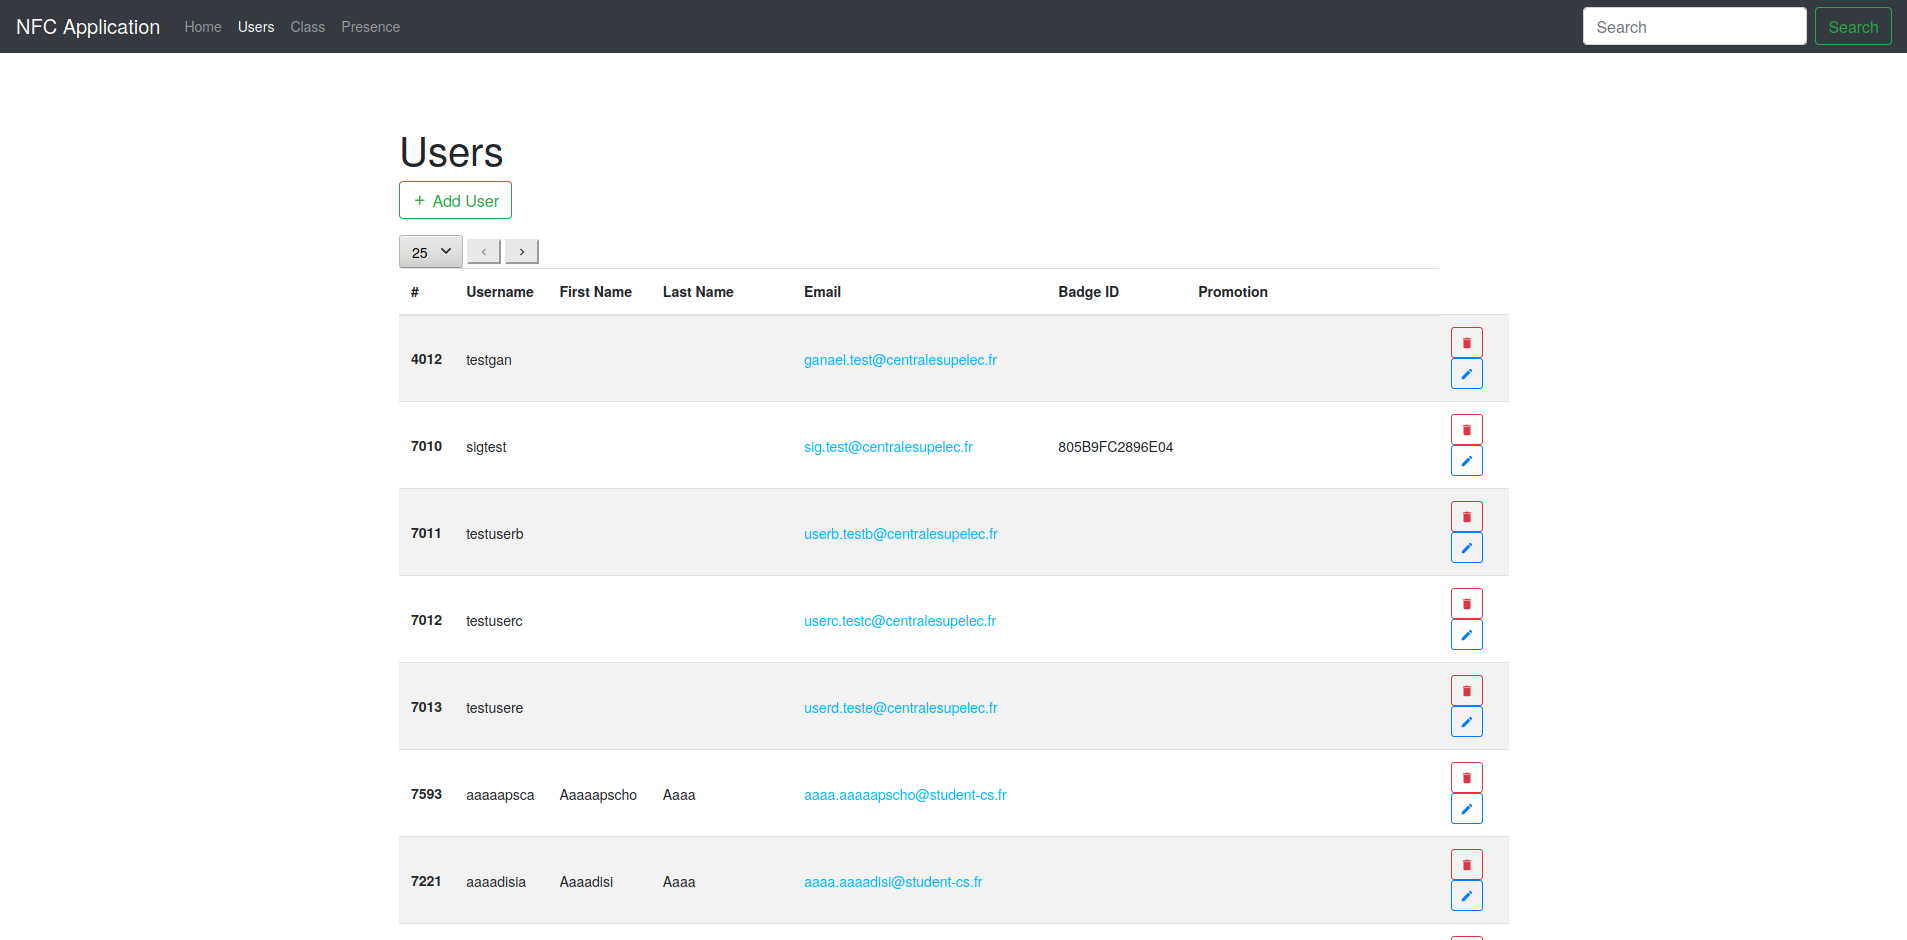
\includegraphics[height=.9\textheight]{../assets/capture_page_users.png}
  \end{figure}
\end{frame}

\begin{frame}
  \begin{figure}
    \centering
    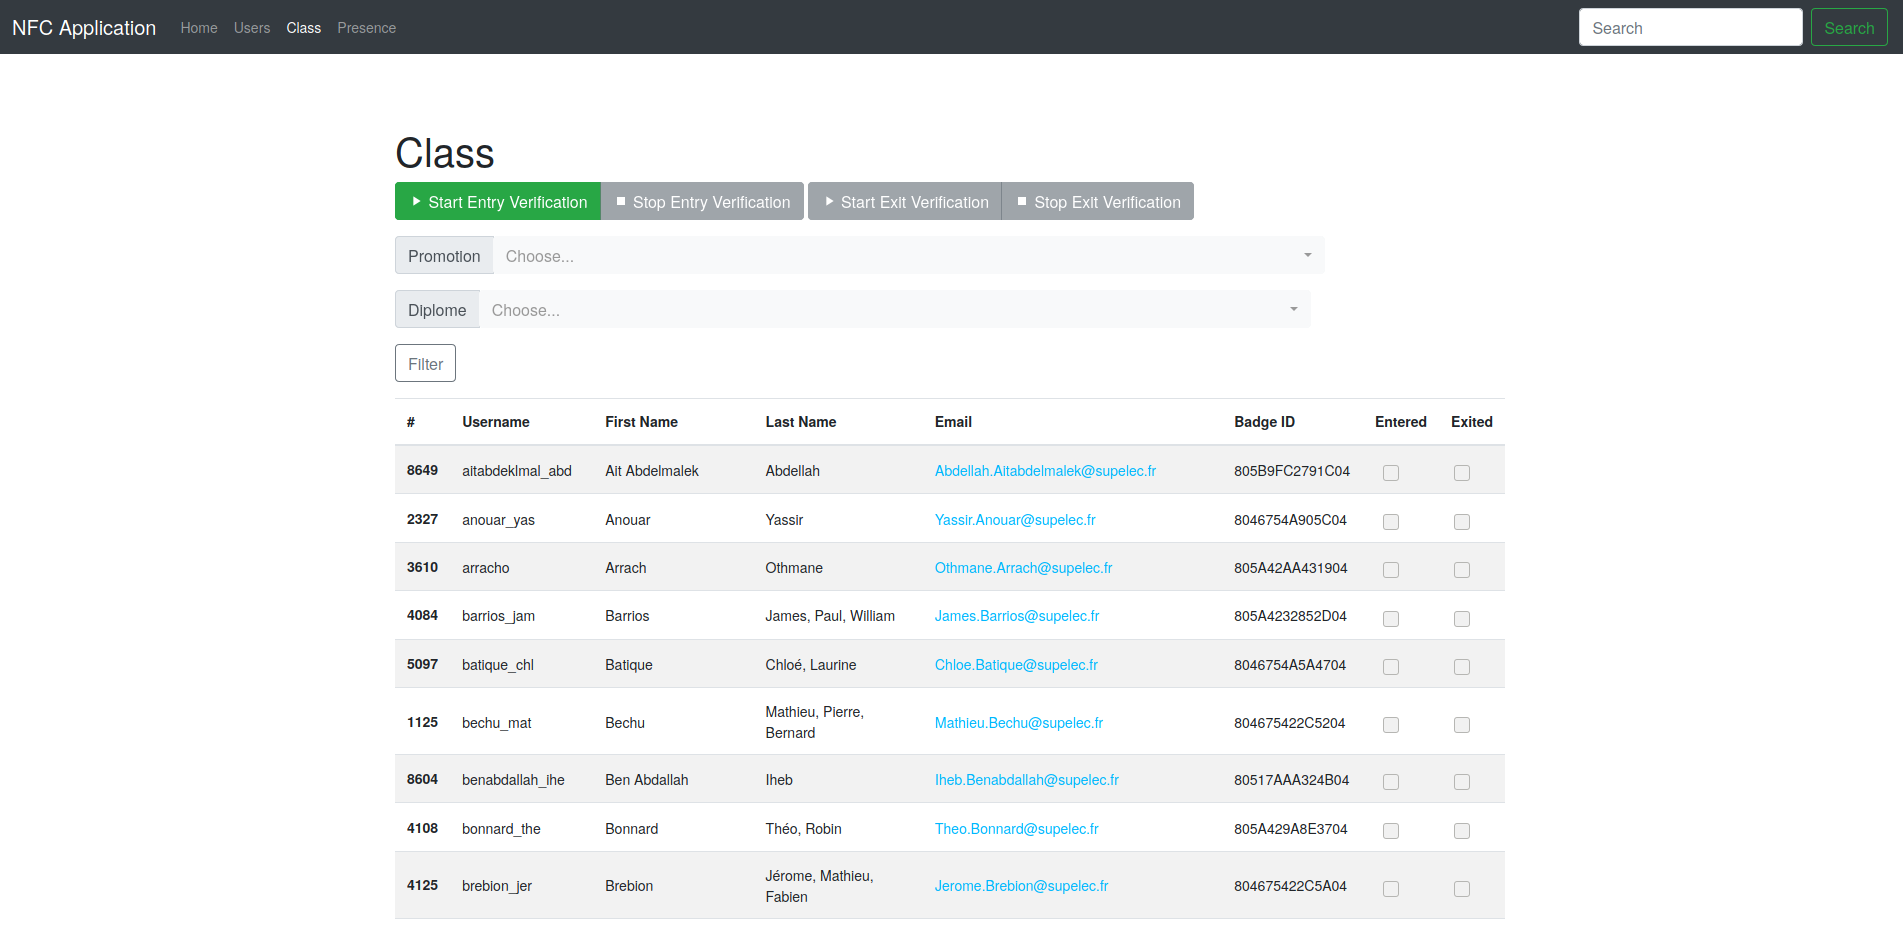
\includegraphics[height=.9\textheight]{../assets/capture_page_class.png}
  \end{figure}
\end{frame}

\begin{frame}
  \begin{figure}
    \centering
    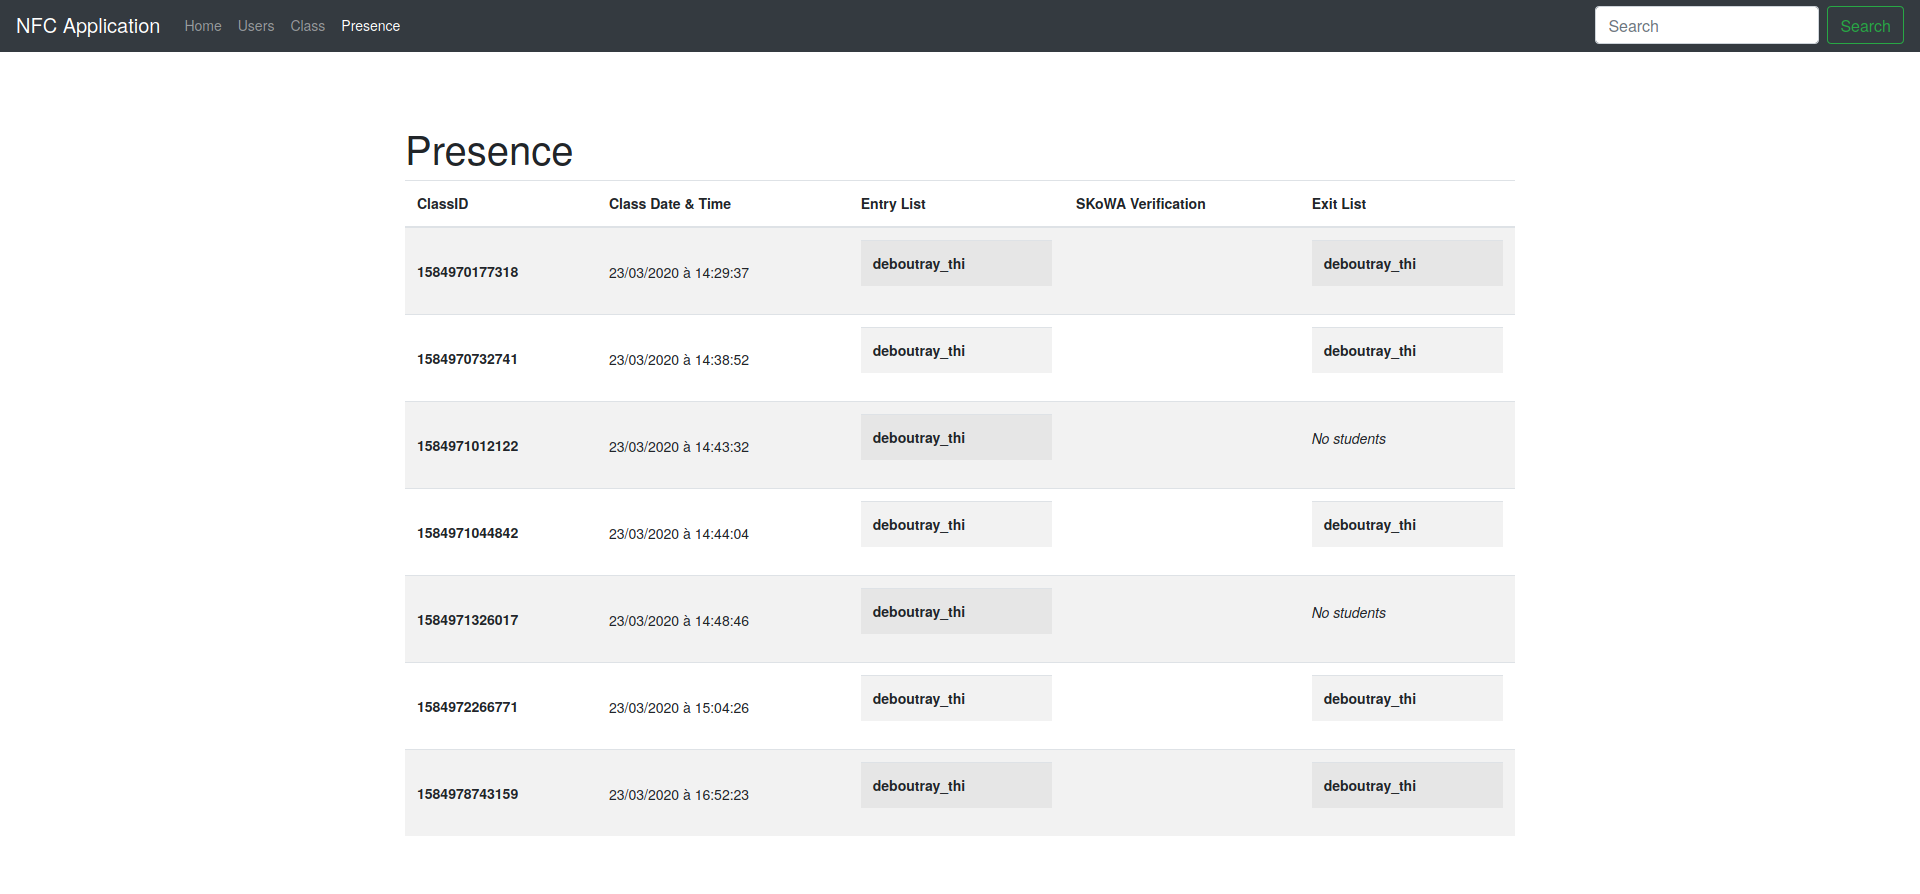
\includegraphics[height=.9\textheight]{../assets/capture_page_presence.png}
  \end{figure}
\end{frame}

\section{Swiss-Knife}

\begin{frame}{Librairie Swiss-Knife : Fonctions abstraites du Tag}
  \centering
  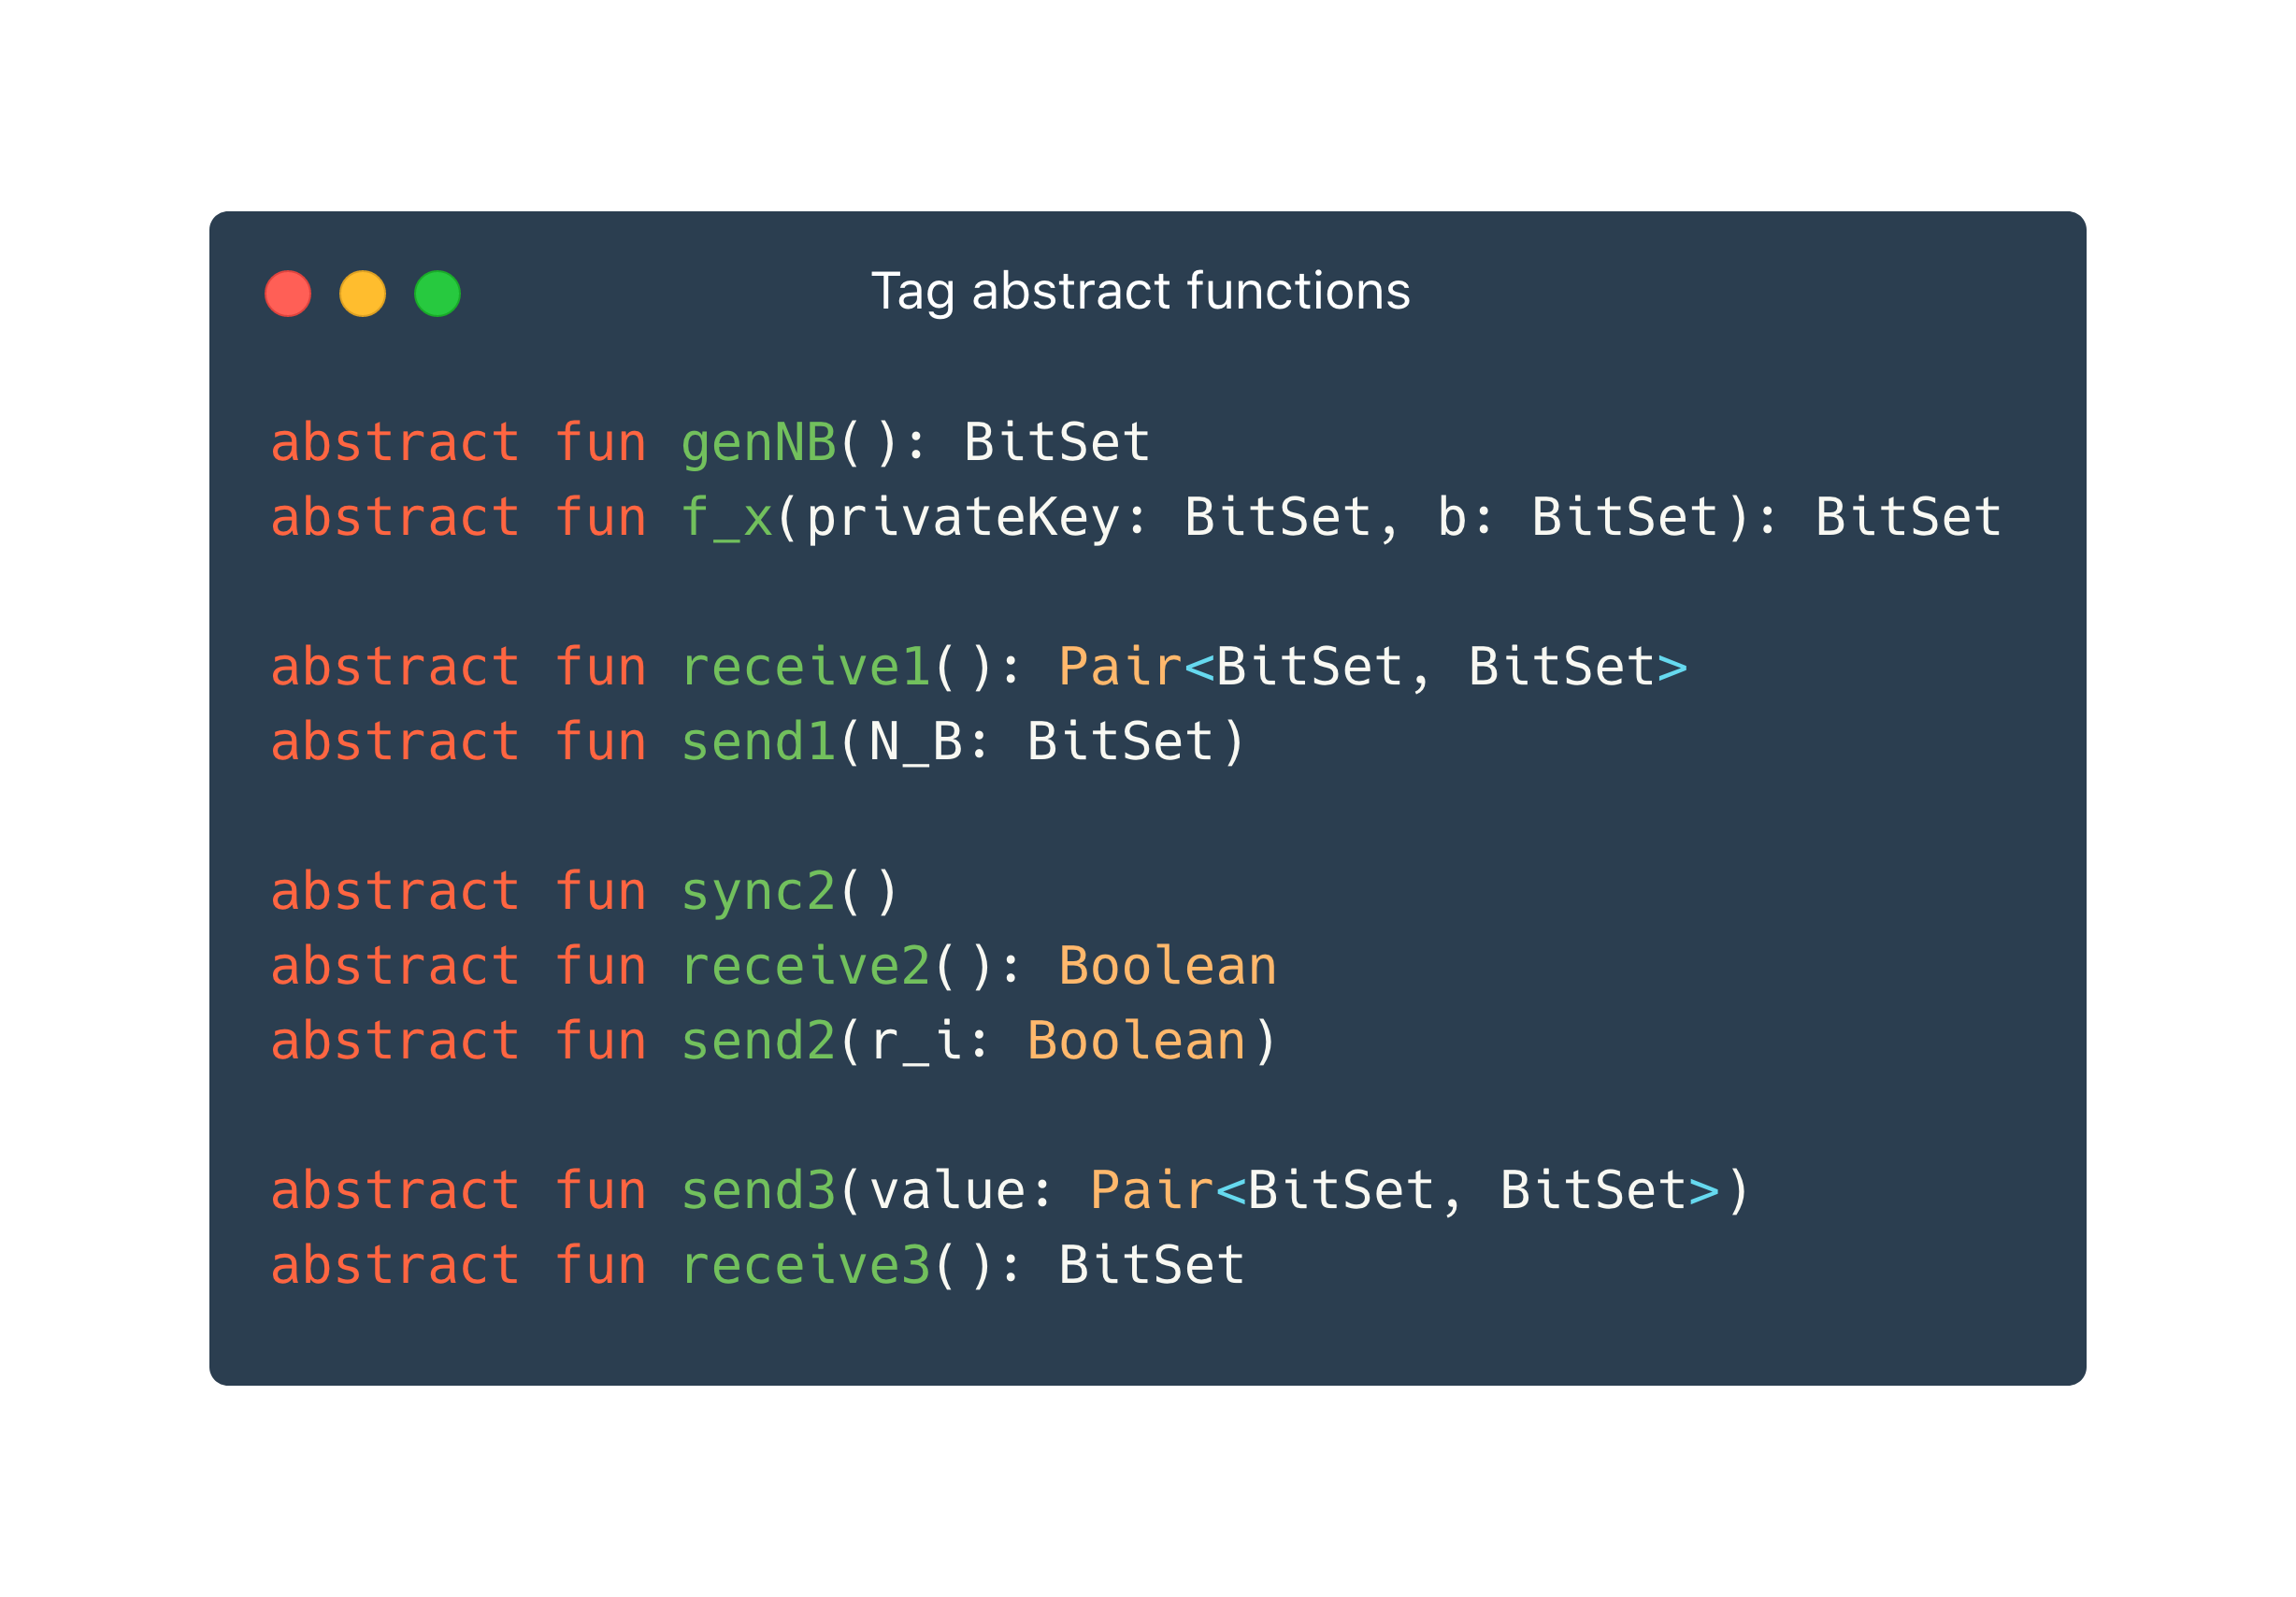
\includegraphics[height=\textheight]{../assets/tagAbs}
\end{frame}

\begin{frame}{Librairie Swiss-Knife : Fonctions abstraites du Reader}
  \centering
  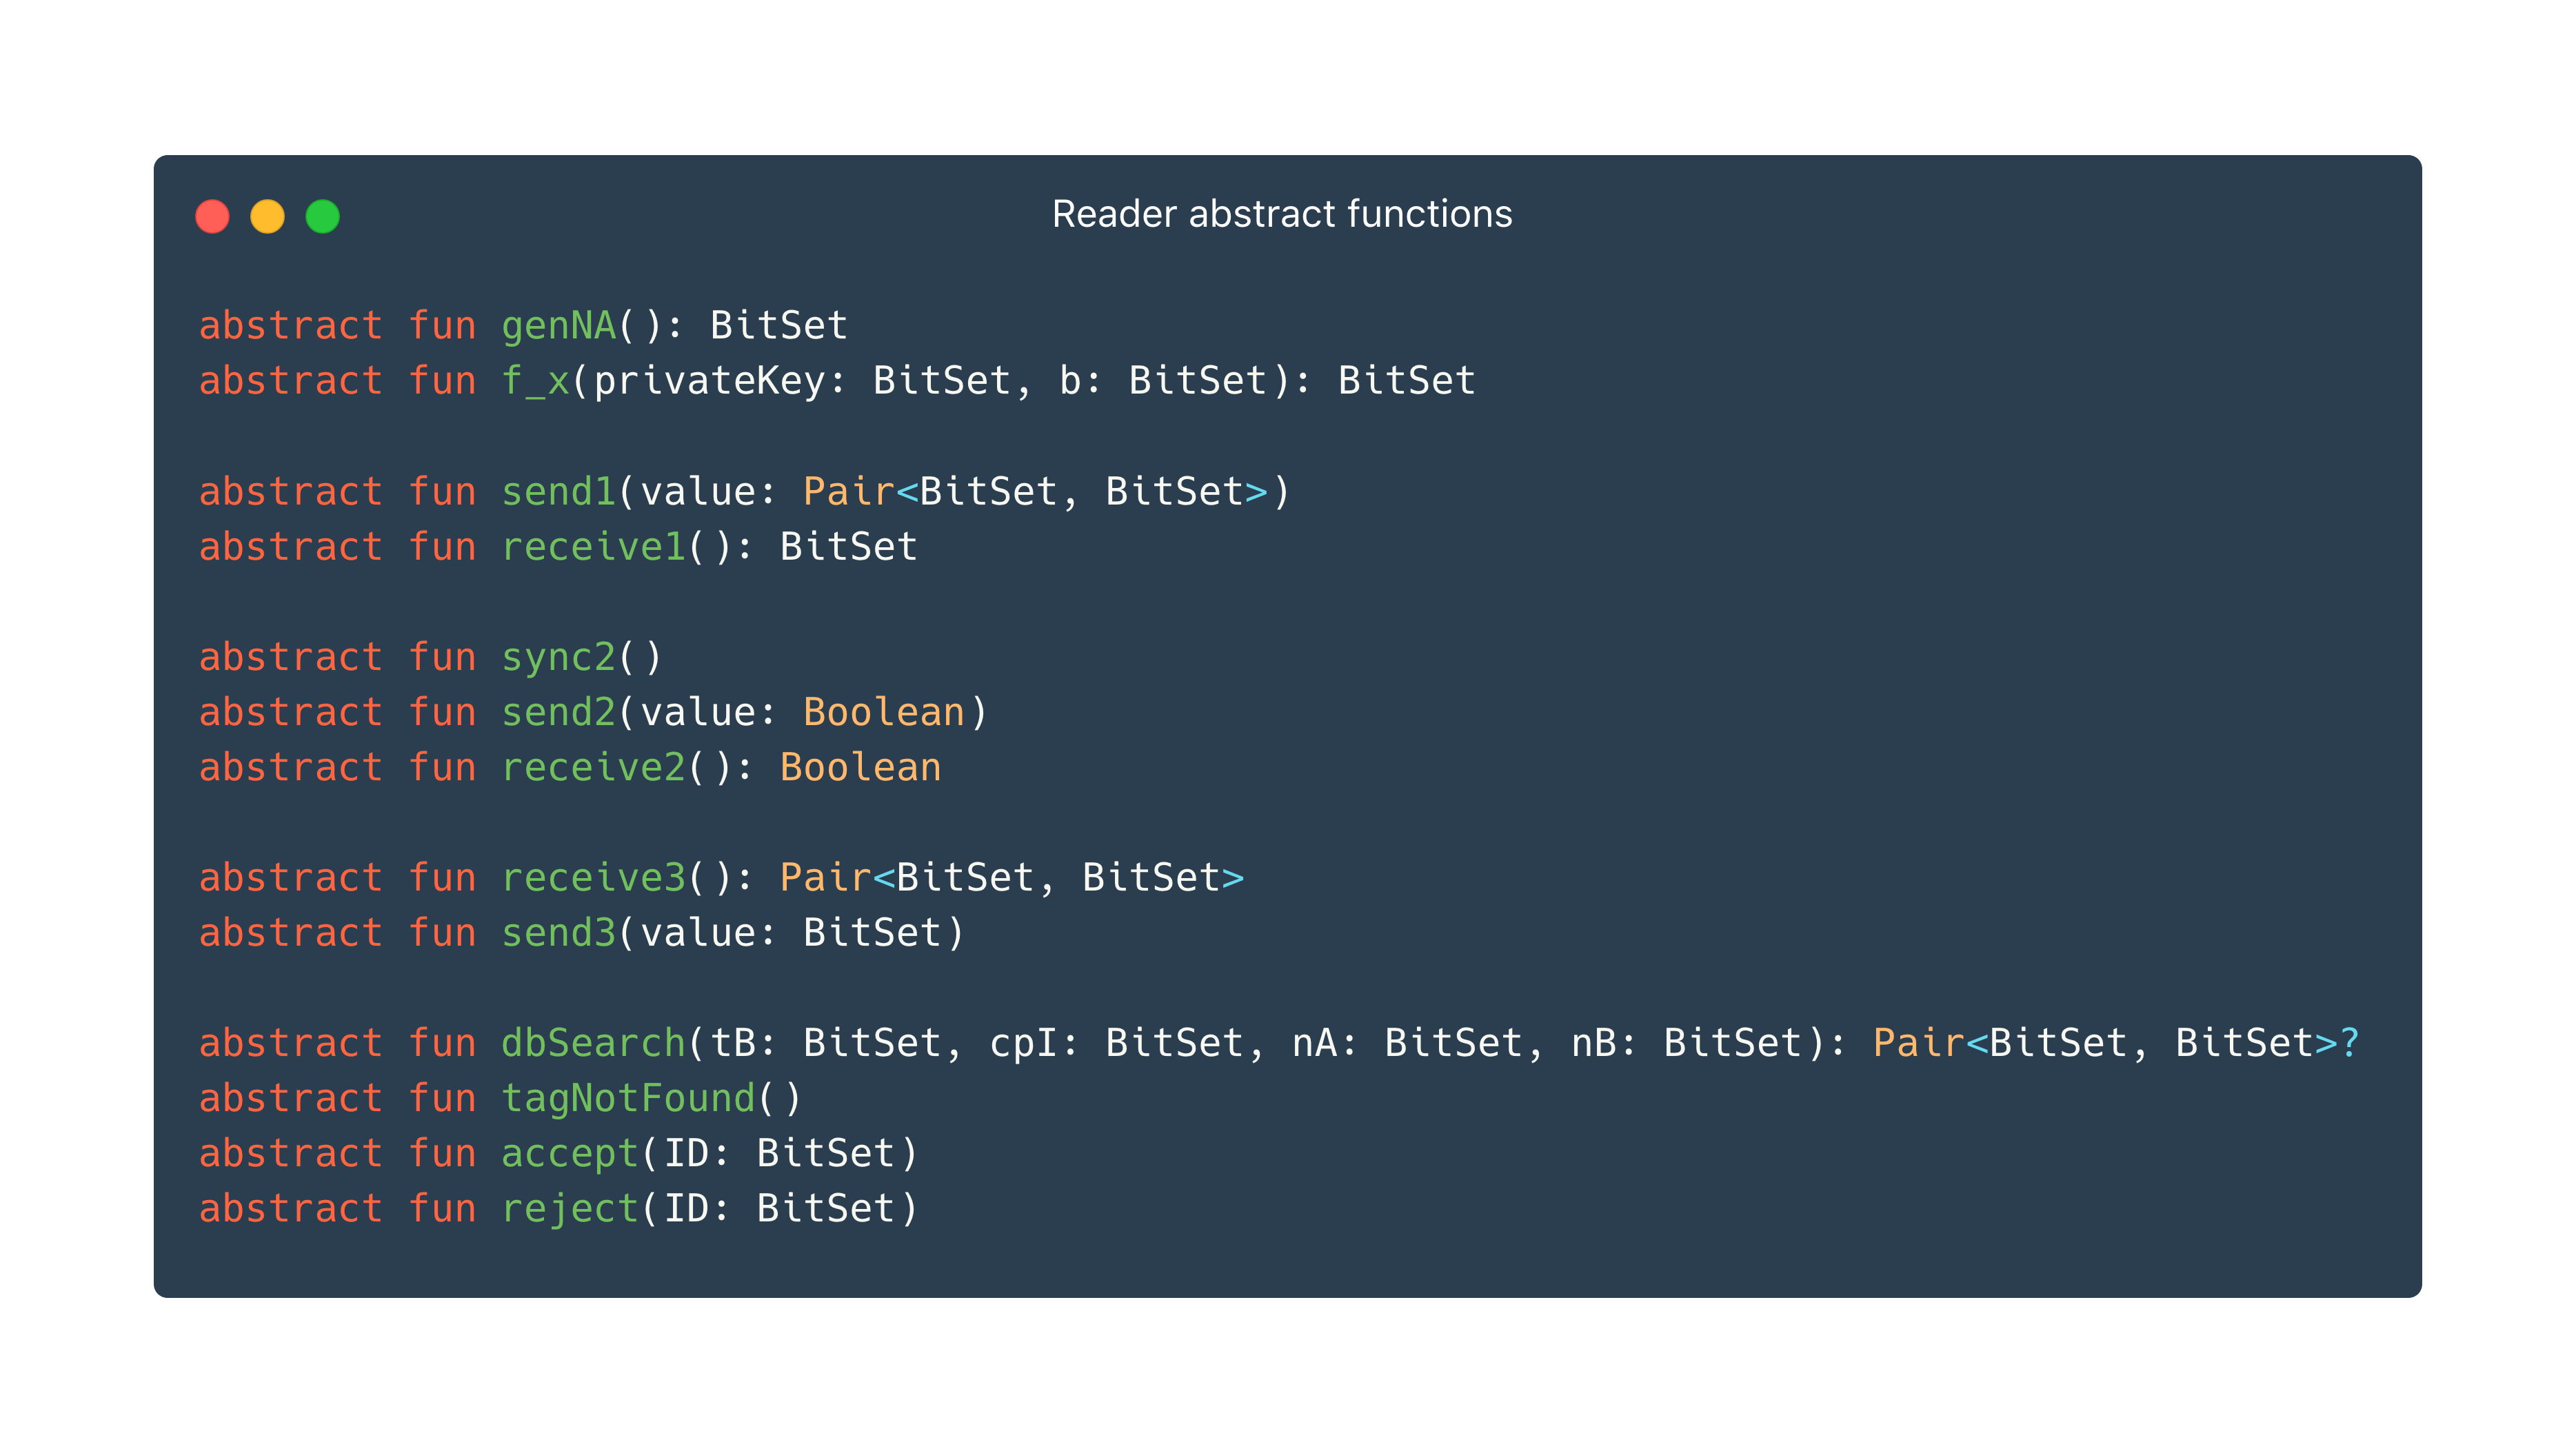
\includegraphics[height=\textheight]{../assets/readerAbs}
\end{frame}

\begin{frame}{Librairie Swiss-Knife : Test unitaire}
  \centering
  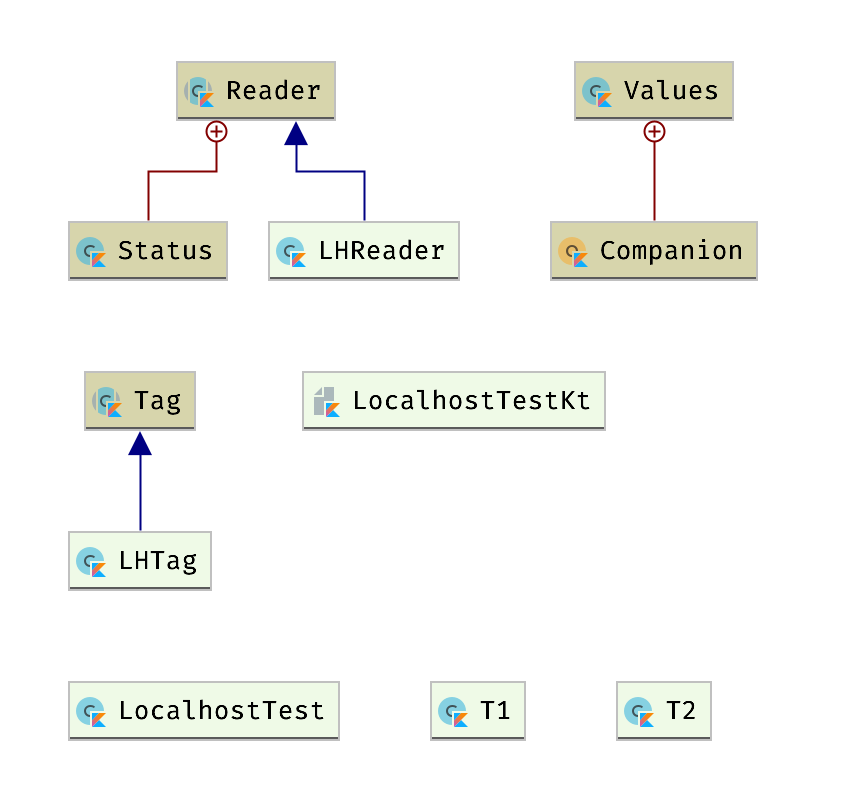
\includegraphics[height=.9\textheight]{../assets/uml_test}
\end{frame}

\section{SKoWA}

\begin{frame}{SKoWA Reader : UML}
  \centering
  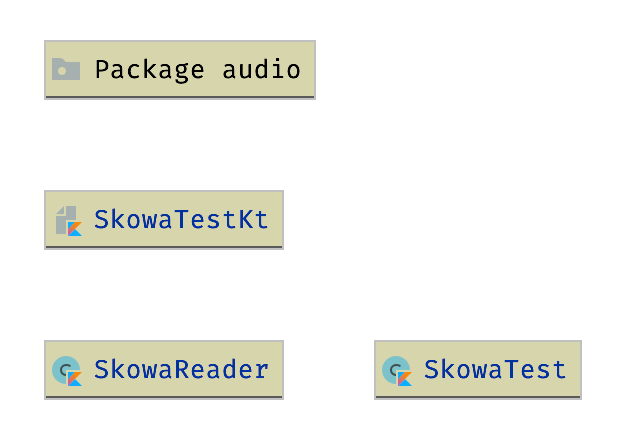
\includegraphics[height=.9\textheight]{../assets/uml_skowa_reader}
\end{frame}

\end{document}
